\documentclass[a4paper, oneside,12pt]{book}
\newcommand{\preprint}{NO}


%% packages utilises
%%---------------------
%\usepackage{etex}


\usepackage[utf8x]{inputenc}
\usepackage[T1]{fontenc}
\usepackage[english, french]{babel}
\usepackage[french]{translator}
\usepackage{frbib}
\usepackage{amsmath}
\usepackage{amssymb}
\usepackage{these}

\usepackage[left=3.5cm, right=2cm, top=2cm, bottom=2cm]{geometry}

\usepackage{ulem}
%\normalem
%\usepackage{rotating}
\usepackage{tabularx}
\usepackage{textcase}
\usepackage{floatflt}
\usepackage{graphicx}
\usepackage{epstopdf}		% .eps to .pdf
\usepackage{moreverb} %% pour le verbatim en boite
\usepackage{multirow} %% pour regrouper un texte sur plusieurs lignes dans une table
\usepackage{url} %% pour citer les url par \url
\urlstyle{sf}
\usepackage[all]{xy} %% pour la barre au dessus des symboles
%\usepackage{shorttoc} %% pour plusieurs tables des matières par la commande \shorttableofcontents{Titre}{profondeur}.
\usepackage{textcomp} %% pour le symbol pour mille par \textperthousand.

%\usepackage[right]{eurosym}

\usepackage{latexsym}
% 
\usepackage{setspace} %allow to change line spacing
\usepackage{fancyhdr} %header / footer
  \setlength{\headheight}{36pt}
\usepackage[ Conny ]{ fncychap }
\usepackage{enumitem} %beautiful enumerations ... no beamer
\usepackage{subfig} %allow to split figure (article / book / report)
\usepackage{caption} %
\usepackage{color} %use color
\usepackage{epsfig,amsfonts} %math mode
\usepackage{array,colortbl} %use array / tabular and apply color / style on them
\usepackage{pstricks} %draw with latex
%\usepackage{tikz}
\usepackage{listings} %source code with avec \being{lstlistgin}

\usepackage{stmaryrd}
%\usepackage{tocbibind}
%\usepackage[nottoc]{tocbibind}
\usepackage{pdfpages}
\usepackage{chngpage}
\usepackage{multicol}
%\usepackage[fit]{truncate}
\pagestyle{fancy}
\fancyhead{} %on efface l'entête

\fancyhead[L]{
\includegraphics[width=1.0cm]{images/esi.jpeg}}
\fancyhead[C]{\scriptsize\textsc{Segmentation Géométrique et Photométrique d’images Acquises par Drones}}
\fancyhead[R]{
\includegraphics[width=1cm]{images/liris.png}}
%\fancyhead[LE,RO]{\nouppercase{\truncate{0.5\headwidth}{\rightmark}}}
%\fancyhead[LO,RE]{\nouppercase{\truncate{0.5\headwidth}{\leftmark}}}
\fancyfoot{}
\renewcommand{\footrulewidth}{1pt}
\fancyfoot[L]{\scriptsize\textbf{DABONNE Hoda}}
\fancyfoot[C]{
\includegraphics[width=1cm]{images/Technidrone.jpg}}
\fancyfoot[R]{\scriptsize\textit\thepage}

%%%%%%%%%%%%%%%%%%%style front%%%%%%%%%%%%%%%%%%%%%%%%%%%%%%%%%%%%%%%%% 
        \fancypagestyle{front}{%
                \fancyhf{}%on vide l'en-tête
                 \fancyfoot[C]{}
                \fancyfoot[R]{\scriptsize \textit\thepage}%
                \fancyfoot[L]{\scriptsize DABONNE Hoda}

                \renewcommand{\headrulewidth}{0pt}%trait horizontal pour l'en-tête
                \renewcommand{\footrulewidth}{1pt}%trait horizontal pour le pied de page
                }
%%%%%%%%%%%%%%%%%%%style main%%%%%%%%%%%%%%%%%%%%%%%%%%%%%%%%%%%%
        \fancypagestyle{*}{%
                \fancyhf{}
                %\renewcommand{\chaptermark}[1]{\markboth{\chaptername\ \thechapter.\ ##1}{}}% redéfinition pour avoir ici les titres des chapitres des sections en minuscules
                \renewcommand{\sectionmark}[1]{\markright{\thesection\ ##1}}
                \fancyhead[c]{\scriptsize\textsc{Segmentation Géométrique et Photométrique d’images Acquises par Drones}}
                \fancyhead[L]{
\includegraphics[width=1.2cm]{images/esi.jpeg}}%
				\fancyhead[R]{
\includegraphics[width=1cm]{images/liris.png}}
				\fancyhead[R]{
\includegraphics[width=1cm]{images/Technidrone.jpg}}

                \fancyfoot[C]{}
                \fancyfoot[R]{\scriptsize \textit\thepage}%
                \fancyfoot[L]{\scriptsize DABONNE HODA}
                }
%%%%%%%%%%%%%%%%%%%style back%%%%%%%%%%%%%%%%%%%%%%%%%%%%%%%%%%%%%%%%%  
        \fancypagestyle{back}{%
                \fancyhf{}%on vide l'en-tête
                \fancyfoot[C]{page \thepage}%
                \renewcommand{\headrulewidth}{0pt}%trait horizontal pour l'en-tête
                \renewcommand{\footrulewidth}{0.4pt}%trait horizontal pour le pied de pages
                }

\usepackage[Algorithme]{algorithm}
\usepackage{algpseudocode}

\usepackage{hyperref}
\usepackage[toc,nonumberlist]{glossaries}
\usepackage{wrapfig}

\usepackage[resetlabels]{multibib}
\newcites{publis}{Publications personnelles}

%% choix des profondeurs de section pour la table des matières
%% 2= subsection, 3=subsubsection
\setcounter{secnumdepth}{2}  %% Avec un numero.
\setcounter{tocdepth}{2}     %% Visibles dans la table des matieres

\makeglossary
\def\underscore{\char`\_}

\usepackage{nomencl}
%\renewcommand{\}{Liste des notations}
%\renewcommand*{\pagedeclaration}[1]{\unskip\dotfill\hyperpage{#1}}
\makenomenclature

\usepackage{makeidx}
\makeindex


\definecolor{colKeys}{rgb}{0,0,1}
\definecolor{colIdentifier}{rgb}{0,0,0}
\definecolor{colComments}{rgb}{0,0.5,1}
\definecolor{colString}{rgb}{0.6,0.1,0.1}

\definecolor{c1}{RGB}{219,144,71}
\definecolor{c2}{RGB}{100,212,78}
\definecolor{c3}{RGB}{255,111,111}
\definecolor{c4}{RGB}{111,139,255}

\definecolor{gris}{gray}{0.45}

\lstset{%configuration de listings
	float=hbp,%
	language=C,
	basicstyle=\ttfamily\small, %
	identifierstyle=\color{colIdentifier}, %
	keywordstyle=\color{colKeys}, %
	stringstyle=\color{colString}, %
	commentstyle=\color{colComments}, %
	columns=flexible, %
	tabsize=3, %
	%frame=trBL, %
	extendedchars=true, %
	%showspaces=false, %
	showstringspaces=false, %
	numbers=none, %
	breaklines=true, %
	breakautoindent=true, %
	captionpos=b,%
	xrightmargin=0cm, %
	xleftmargin=0cm,
	mathescape=true
}


\frenchspacing

\newgeometry{hmargin={0pt,0pt},vmargin={0pt,0pt}}
\savegeometry{include}

\newgeometry{vmargin={4.1cm,3.6cm},hmargin={3cm,2cm},twoside}
\setstretch{1.1}
\savegeometry{normalpreprint}

\newgeometry{vmargin={4.1cm,3.6cm},hmargin={2cm,3cm},twoside}
\setstretch{1.1}
\savegeometry{normalpreprintinverse}

\newgeometry{vmargin={4.1cm,3.6cm},hmargin={2.5cm,2.5cm}}
\setstretch{1.1}
\savegeometry{normaldigital}

\ifthenelse{\equal{\preprint}{YES}}
{
\loadgeometry{normalpreprint}
\savegeometry{normal}
\loadgeometry{normalpreprintinverse}
\savegeometry{normalinverse}
}
{
\loadgeometry{normaldigital}
\savegeometry{normal}
\savegeometry{normalinverse}
}


%%%%%%%%%%%%%%%%%%%%%%%%%%%%%%%%%%%%%%%%%%%%%%%%%%%%%%%%%%%%%
%	SubFloat environment for lstlisting inside subloat		%
%%%%%%%%%%%%%%%%%%%%%%%%%%%%%%%%%%%%%%%%%%%%%%%%%%%%%%%%%%%%%

\captionsetup[subfloat]{
}

\makeatletter
\newbox\sf@box
\newenvironment{SubFloat}[2][]%
	{	\def\sf@one{#1}%
		\def\sf@two{#2}%
		\setbox\sf@box\hbox
			\bgroup}%
	{	\egroup
	\ifx\@empty\sf@two\@empty\relax
		\def\sf@two{\@empty}
	\fi
	\ifx\@empty\sf@one\@empty\relax
		\subfloat[\sf@two]{\box\sf@box}%
	\else
		\subfloat[\sf@one][\sf@two]{\box\sf@box}%
	\fi}
\makeatother

\usepackage{bibentry}
\nobibliography*

%% macro/racourcis por les symboles et commandes usuelles
%%%%%%%%%%%%%%%% environnement pour les résumés%%%%%%%%%%%%%%%%%%%%
\makeatletter
\newenvironment{abstract}{%
    \null\vfil
    \@beginparpenalty\@lowpenalty
    \begin{center}%
            \@endparpenalty\@M
    \end{center}}%
   {\par\vfil\null}
\makeatother
% macro pour le 'debuggage': permet de corriger le document avec plus de facilit�
\newcommand{\mydebuglabel}[1]{\label{#1}}
%\newcommand{\debuglabel}[1]{\label{#1}}

% nouveaux environements de theoreme
%----------------------
\newtheorem{proposition}{Proposition}
%\newtheorem{lemme}{Lemme}
\newtheorem{exemple}{Exemple}
%\newcommand{\mydefinition}[2]{\begin{definition}{\bf #1:} #2$\diamond$\end{definition}}
%\newcommand{\mydefinition}[1]{\begin{definition}#1\end{definitio\newtheorem{theoreme}{Theorem}[section]
\newcommand{\deftitle}[1]{\begin{definition}{\bf (#1)}}

% alias de notation mathematiques
%-----------------------
%%%% debut macro %%%% %\newcommand{\barre}[1]{#1}  %% pour ajouter une barre horizontale au dessus d'un symbole

%\newcommand{\vector}[1]
%{\mathchoice
%{\overset{\mbox{\xymatrix{*{\hphantom{\displaystyle #1}}
%\ar[]+L;[]+R}}}{\displaystyle #1}}%
%{\overset{\mbox{\xymatrix{*{\hphantom{\textstyle #1}}
%\ar[]+L;[]+R}}}{\textstyle #1}}%
%{\overset{\mbox{\xymatrix{*{\hphantom{\scriptstyle #1}}
%\ar[]+L;[]+R}}}{\scriptstyle #1}}%
%{\overset{\mbox{\xymatrix{*{\hphantom{\scriptscriptstyle #1}}
%\ar[]+L;[]+R}}}{\scriptscriptstyle #1}}% 
%}

\newcommand{\barre}[1]{\overline{#1}}%% pour ajouter une barre horizontale au dessus d'un symbole
\newcommand{\prosite}[1]{{\bf{\small#1}}}%% pour �crire des motifs prosite
\newcommand{\permille}{\hbox{$\,^0\!/_{00}$}}%% symbole pourmille


%Pour changer la distance de la fl�che, on peut proc�der ainsi.
%\renewcommand{\ra}[1]
%{\overset{\raisebox{-1pt}{\mbox{\xymatrix{*{\hphantom{#1}}
%\ar[]+L;[]+R}}}}{#1}}
%%%% fin macro %%%%


%% alias specifiques pour les relations, utilisables seulement en mode mathematique
%-----------------------
\newcommand{\La}{\ensuremath{\langle}}
\newcommand{\Ra}{\ensuremath{\rangle}}

\newcommand{\dcp}[2]{\parallel_p^{\La #1,#2 \Ra}}
\newcommand{\dcs}[2]{\parallel_s^{\La #1,#2 \Ra}}
\newcommand{\cp}[2]{\parallel_p^{#1,#2}}
\newcommand{\cs}[2]{\parallel_s^{#1,#2}}
\newcommand{\cscc}{\parallel_s^{c_1,c_2}} % racourci pour cs avec comme classe c1 et c2
\newcommand{\scp}{\parallel_p} % scp pour Simple Common Prefix (simple = pas de classe)
\newcommand{\scs}{\parallel_s} % scs pour Simple Common Suffix (simple = pas de classe)
%\newcommand{\inc}[2]{\not\sim^{#1,#2}}
\newcommand{\sinc}{\parallel_s^{\neq}} % sinc pour Simple Incompatible (simple = pas de classe)
\newcommand{\stc}{\scs} % stc: suffixe toute classe
\newcommand{\scce}{\parallel_s^{ce}} % scce: suffixe commun de contre exemple
%\newcommand{\cp}[2]{{\vphantom{\parallel_p^{#2}}}^{#1}{\parallel_p^{#2}}}
%\newcommand{\cs}[2]{{\vphantom{\parallel_s^{#2}}}^{#1}{\parallel_s^{#2}}}

\newcommand{\suff}[2]{\text{{\it Suff}}_{#1}(#2)}
\newcommand{\pref}[2]{\text{{\it Pref}}_{#1}(#2)}
\newcommand{\relalias}{\ifmmode{\parallel_{r}}\else{$\parallel_{r}$}\fi} % un symbol pour repr�senter une relation qque entre 2 etats

%% alias pour la definition des classes d'automates, des acceptations et des automates particuliers (en mode math ou non)
%-----------------------
\newcommand{\assurepasmath}[1]{\ifmmode\text{#1}\else #1\fi}
%\newcommand{\cnfa}{\ifmmode\text{NFAC}\else NFAC}
\newcommand{\ufa}{\assurepasmath{UFA}}
\newcommand{\ufas}{\assurepasmath{UFAs}}
\newcommand{\dfa}{\assurepasmath{DFA}}
\newcommand{\dfas}{\assurepasmath{DFAs}}
\newcommand{\nfa}{\assurepasmath{NFA}}
\newcommand{\nfas}{\assurepasmath{NFAs}}
\newcommand{\rfsa}{\assurepasmath{RFSA}}
\newcommand{\rfsas}{\assurepasmath{RFSAs}}
\newcommand{\kamb}[1]{\ifmmode\text{AFA}_{#1}\else AFA\ensuremath{_{\text{#1}}}\fi}
\newcommand{\cnfa}{\assurepasmath{{NFC}}}
\newcommand{\cnfas}{\assurepasmath{{NFCs}}}
\newcommand{\cdfa}{\assurepasmath{{DFC}}}
\newcommand{\cdfas}{\assurepasmath{{DFCs}}}
\newcommand{\cufa}{\assurepasmath{{UFC}}}
\newcommand{\cufas}{\assurepasmath{{UFCs}}}
\newcommand{\ckamb}[1]{\ifmmode\text{{AFC}}_{#1}\else {AFC}\ensuremath{_{\text{#1}}}\fi}

\newcommand{\Sa}{\ifmmode\mathcal{S}\else\ensuremath{\mathcal{S}}\fi}

\newcommand{\auset}[2]{\ifmmode\boldsymbol{D}_{#1}(#2)\else\ensuremath{\boldsymbol{D}_{\text{#1}}(\text{#2})}\fi}
\newcommand{\partitions}[1]{\ifmmode\boldsymbol{P}(#1)\else\ensuremath{\boldsymbol{P}}(#1)\fi}
% ensemble des partitions restreinte a une classe d'automate
%\newcommand{\partitionsr}[2]{\ifmmode\mathcal{P}art_{#1}(#2)\else\ensuremath{\mathcal{P}art_{#1}}(#2)\fi}
\newcommand{\partitionsr}[2]{\ifmmode\boldsymbol{P}_{#1}(#2)\else\ensuremath{\boldsymbol{P}_{#1}}(#2)\fi}

\newcommand{\Acc}[2]{\ifmmode Acc_{#1}(#2)\else\ensuremath{Acc_{\text{#1}}(\text{#2})}\fi}
\newcommand{\smca}[1]{\ensuremath{\text{{\it MCA}}(}#1\ensuremath{)}}
\newcommand{\mca}{\ensuremath{\text{{\it MCA}}}} % mca sans le sample
\newcommand{\ua}{\ensuremath{\text{{\it UA}}}}
\newcommand{\sua}[1]{\ensuremath{\text{{\it UA}}(}#1\ensuremath{)}}
\newcommand{\mcak}[1]{\ensuremath{\text{{\it MCA}}_{#1}}}
\newcommand{\smcak}[2]{\ensuremath{\text{{\it MCA}}_{#1}(}#2\ensuremath{)}}
\newcommand{\smcau}[1]{\smcak{u}{#1}}
\newcommand{\mcau}{\mcak{u}}
\newcommand{\pta}{\ensuremath{\text{{\it PTA}}}}
\newcommand{\spta}[1]{\ensuremath{\text{{\it PTA}}(}#1\ensuremath{)}}
\newcommand{\au}[1]{\ensuremath{\La\Sigma,\Gamma_{#1},Q_{#1},I_{#1},\delta_{#1},\rho_{#1}\Ra}}% automate classifieur
\newcommand{\nau}[1]{\ensuremath{\La\Sigma,Q_{#1},I_{#1},\delta_{#1},F_{#1}\Ra}}% automate normal

%% alias des op�rateurs de parcours
%---------------------------------
% seulement en mode math !!!
% fusion simple sur partition
\newcommand{\ispar}{\prec} % inf�riorit� stricte
\newcommand{\ipar}{\prec^*} % inf�riorit�
\newcommand{\fuspar}{\xrightarrow{\prec}} % op�rateur de fusion
%\newcommand{\fispar}{\xrightarrow{\succ}}% op�rateur de fission
% fusion simple sur automates
\newcommand{\isaut}{\prec_{A}} % inf�riorit� stricte
\newcommand{\iaut}{\prec^*_{A}} % inf�riorit�
\newcommand{\fusaut}{\xrightarrow{\prec_A}}% op�rateur de fusion simple
\newcommand{\fisaut}{\xrightarrow{\succ_A}}% op�rateur de fission simple
\newcommand{\fussaut}{\xrightarrow{A*}}% op�rateur de suite de fusion simples
% fusion deterministe
\newcommand{\idet}{\prec^*_{det}}
\newcommand{\isdet}{\prec_{det}}
\newcommand{\fdet}{\xrightarrow{det}}
% fusion restreinte au determinisme
\newcommand{\irdet}{\prec^*_{D}}
\newcommand{\isrdet}{\prec_{D}}
\newcommand{\frdet}{\xrightarrow{D}}
% fusion desambiguisante
\newcommand{\ides}{\prec^*_{des}}
\newcommand{\isdes}{\prec_{des}}
\newcommand{\fdes}{\xrightarrow{des}}
% fusion restreinte a la k-ambiguite
\newcommand{\ikam}[1]{\prec^*_{#1-amb}}
\newcommand{\iskam}[1]{\prec_{#1-amb}}
\newcommand{\fkam}[1]{\xrightarrow{#1-amb}}

%% alias de presentation
%-----------------------
\newcommand{\etc}{etc.}
%\newcommand{\commentaire}[1]{{\tiny #1}}
\newcommand{\commentaire}[1]{}
\newcommand{\proof}[1]{{\bf Preuve:} #1}
%\newcommand{\proof}[1]{{\bf Proof:} #1$\square$}
\newcommand{\hintproof}[1]{{\bf Id�e de la preuve:} #1}
%\newcommand{\hintproof}[1]{{\bf Hint of the proof:} #1$\square$}
%\newcommand{\mycaption}[1]{\caption{{\small #1}}}
%\newcommand{\mycaption}[1]{\caption{ #1}}

%\newcommand{\remark}[1]{{\small Remark: \emph{#1}}}
\newcommand{\remark}[1]{Remark: \emph{#1}}

\newcommand{\resumefr}[1]{%
\thispagestyle{empty}
\section*{R�sum�}
#1 
\vfill
}

% >> macro pour la separation d'un bout de page en deux parties, utile pour les figures et leur caption a droite ou gauche
% l'argument specifie la taille de la partie gauche
\newlength\jataille
\newcommand{\figgauche}[3]%
{\jataille=\textwidth\advance\jataille by -#1
\parbox{#1}{#2}
\parbox{\jataille}{#3}
}

\newcommand{\figtxt}[1]%
{{\it {\small #1}}}
% << fin macro

% >> macro pour tracer un trai horizontal sur la largeur de la page
\newcommand{\traithoriz}{\raisebox{0.4em}{\vrule depth 0pt height 0.4pt width \textwidth}}


% nom des algos
\newcommand{\edsm}{EDSM}
\newcommand{\rpni}{RPNI}
\newcommand{\edsmdfaf}{D$_{\text{f}}$\textit{edsm}}
\newcommand{\edsmdfac}{D$_{\text{c}}$\textit{edsm}}
\newcommand{\hcdfaf}{D$_{\text{f}}$\textit{hc}}
\newcommand{\hcdfac}{D$_{\text{c}}$\textit{hc}}
\newcommand{\hcufaf}{U$_{\text{f}}$\textit{hc}}
\newcommand{\hcufac}{U$_{\text{c}}$\textit{hc}}
\newcommand{\delete}{DLT2}
\newcommand{\majvote}{MAJ}


\newcommand{\kcite}[1]{
\begin{verse}
\cite{#1}~\bibentry{#1}
\end{verse}
}
%\newcommand{\kcite}[1]{\cite{#1}}

%%%% debut macro pour faire des lignes �paisses dans les tableaux %%%%
\makeatletter
\def\hlinewd#1{%
\noalign{\ifnum0=`}\fi\hrule \@height #1 %
\futurelet\reserved@a\@xhline}
\makeatother
%%%% fin macro %%%%


%%%%%%%%%%%%%%%%%%%%%%%%%%%%%%%%%%%%%%%%%%%%%%%%%%%%%%%%%%
%%%%%%%%%%%%%%%%%		Exemple		%%%%%%%%%%%%%%%%%%%%%%
%%%%%%%%%%%%%%%%%%%%%%%%%%%%%%%%%%%%%%%%%%%%%%%%%%%%%%%%%%

% glossary entry : defines the identifier in the glossary table (1rst arg), 
% and the description in second arg.
\newglossaryentry{id}{
name={ID}, %what appear in text
description={\emph{Identifier} : Identifiant}, %what appear in glossary
first={ID (\emph{Identifier} : Identifiant)}} %what appear the first time in text
\newcommand{\id}{\gls{id}} % shortcut pour the glossary entry. Simply coll \id in the text
\newcommand{\ID}{ID} % to put the text without using the glossary shortcut.


\newglossaryentry{sg}{
name={SG}, %what appear in text
description={Société Générale}, %what appear in glossary
first={SG ( Société Générale)}} %what appear the first time in text
\newcommand{\sg}{\gls{sg}} % shortcut pour the glossary entry. Simply coll \id in the text

\newglossaryentry{sgbf}{
name={SGBF}, %what appear in text
description={Société Générale Burkina Faso}, %what appear in glossary
first={SGBF ( Société Générale Burkina Faso)}} %what appear the first time in text
\newcommand{\sgbf}{\gls{sgbf}} % shortcut pour the glossary entry. Simply coll \id in the text




%%  1ere de Couverture (titre sur une seule ligne latex)
\titre{Mémoire de fin de cycle master SI-SAD}

\soutenue
%%   Laisser cette ligne en commentaire sauf pour la version finale.
%%   (la premiere page contiendra "a soutenir le ..."
%%   au lieu de "soutenue le ...")


%% Les différents champs de la couverture...
\datesout{`` fin 20xx ''}
\Auteur{Hoda}{DABONNE}%sur une seule ligne latex

\ecole{Ecole Supérieur d'Informatique}  % { rennes1 | insa | ens }
\Labo{Lab.}
\Umr{XXXX}
\LaboEtendu{Laboratoire de recherche} % sauf INSA
\ComposanteUniversitaire{Université Nazi Boni} % sauf INSA

%% La composition du jury : prénom, nom, titre
\President[Mme]{Prenom}{Nom}{Titre} %% le président du jury
\Rapporteur{Prenom}{Nom}{Titre}
\Rapporteur[Mme]{Prenom}{Nom}{Titre}
%% Si vous avez N rapporteurs ça marche toujours...
\Examinateur[Mme]{Prenom}{Nom}{Titre}
\Examinateur{Prenom}{Nom}{Titre}
%% idem...
\Advisor{Serge}{Miguet}{Maitre de Conférences}
\Advisor{Prénom}{Nom}{Titre}

\Mention{Thèmatique}
\Keywords{Mots clés}
\ordre{00000}    %% le numéro d'ordre donné par la Scol.


\title{\TITRE}

\author{\AUTp \AUTn}

\hypersetup{
	pdfauthor={{\AUTp} {\AUTn}},
	pdftitle={{\TITRE}},
	pdfsubject={\MENTION},
	pdfkeywords={\KEYWORDS},
	hidelinks
}

\begin{document}
\frontmatter

\loadgeometry{include}
\addtocounter{page}{-1}
\thispagestyle{empty}
\begin{center}

\includegraphics[width=\textwidth]{miscpages/title.pdf}
\end{center}
\newpage
\thispagestyle{front}


\loadgeometry{normalinverse}
% \addtocounter{page}{-1}
\ifthenelse {\equal{\ISDEF}{0}}
{} {
\thispagestyle{front}
%\addtocounter{page}{1}



% ------------------------------% ------------------------------%
\chapter*{Avant propos}
%\addcontentsline{toc}{chapter}{Avant propos}
\markboth{Avant propos}{Avant propos}
% ------------------------------% ------------------------------%
L’Université Nazi BONI a été créée le 23 mai 1997. Elle est située à quinze
(15) kilomètres à l’Ouest de Bobo et est composée de six (06) établissements à savoir :
\begin{itemize}
  \item L'Ecole Supérieure d'Informatique(ESI)
  \item L'Institut de Développement Rural(IDR)
  \item l'Institut Nationale des Sciences de la Santé(INSSA)
  \item l'Institut Universitaire de Technologie(IUT)
  \item l'UFR Sciences Juridique Politique Economique et Gestion(UFR SJPEG)
  \item l'UFR Sciences et Technologies(UFR ST)
  \item l'UFR Sciences Humaines, Lettres, Arts, et Communication(UFR SH-LAM)
\end{itemize}

L'ESI a pour mission d'accompagner le Burkina Faso dans sa transformation
digitale. Pour cela, elle forme depuis sa création des cadres supérieurs en
informatique qui font sa fierté dans toutes le administrations du pays.

Afin de préparer les futurs diplômés à l’insertion dans la vie professionnelle,
l'ESI prévoit que chaque futur diplômé effectue un stage de fin de cycle
dans une entreprise ou dans un centre de recherche ou de développement.

C’est dans ce contexte, que nous avons été reçu au LIRIS pour notre stage de fin de cycle.
Le présent document fait office de memeoire des travaux que nous y avons menés.

\thispagestyle{front}
%\addtocounter{page}{2}
%%  une page de citation (pas indispensable)
 \vspace{\stretch{1}}
\vspace{0.5\linewidth}
\begin{flushright}
  %\emph{No physical quantity can continue to change exponentially forever. Your job is delaying forever.}\\
  \emph{}\\
  
\end{flushright}
\vspace{\stretch{2}}

%% Encore une page blanche pour que les remerciements arrivent
%%  sur une page impaire

\thispagestyle{front}
%\addtocounter{page}{3}
\chapter*{Dédicace}

\vspace*{\stretch{1}}
\begin{flushright}
  A  \\
  Mes parents\\
  \textbf{Monsieur \textsc{DABONNE} Hanido}\\ Et  \\
  \textbf{Madame \textsc{DABONNE} Née BALIMA Habibou}\\
  \normalsize Je ne vous remercirais jamain assez pour tout ce que vous avez fais 
  pour moi au quotidient. Soyez en remercier\\
  \textbf{Madame \textsc{DABONNE} née \textsc{COMOE} Maouwa}\\
  \normalsize Que ton ame repose en paix. 


  A ma bousole  \\
  \textbf{Monsieur \textsc{DABONNE} Ousseni}\\
  \normalsize Ton acharmement et ta determination au travail font de toi ma source
   d'inspiration et mon modèle. Merci de toujours me montrer le chemain de la droiture.
\end{flushright}

\vspace*{\stretch{2}}

\thispagestyle{front}
%\addtocounter{page}{4}

%\remerciements
\chapter*{Remerciements}

La redaction de ce memoire a été possible grace a plusieures personne et institution à qui je voudrais 
temoigner ma gratitude et mes sincères reconnaissances:

  Je tiens à remercier le programme Erasmus+
  pour m'avoir donner cette chance de sejourner en France et de faire mon stage 
  dans l'un des plus grands laboratioire francais. 
  
  
  Je remercier \textbf{Professeur Serge \textsc{Miguet}} et \textbf{Professeur Mihaela \textsc{Scuturici}}
    mes tuteur de stage, pour les conseils et suggestions, combien précieux dans la
    réalisation de notre travail;
  
  Je desire remercier \textbf{Professeur Tigiane\textsc{Yelemou}} mon tuteur accademique
  pour ces conseils et suggestions.
 
  Un grand merci à \textbf{Professeur Pasteur \textsc{Poda}}, coordonateur de notre master
    pour son don de soit dans le bon deroulement de notre formation.

  En fin, je tien à remercier l'ensemble du corps professoral et administratif de l'ESI  pour toute la
    disponibilité et l'encadrement dont nous avons bénéficié.
  
A tous ceux qui ont contribué d'une manière ou d'une autre à la réalisation de
ce travail, MERCI.

\thispagestyle{front}
%\addtocounter{page}{5}
}

\begin{center}
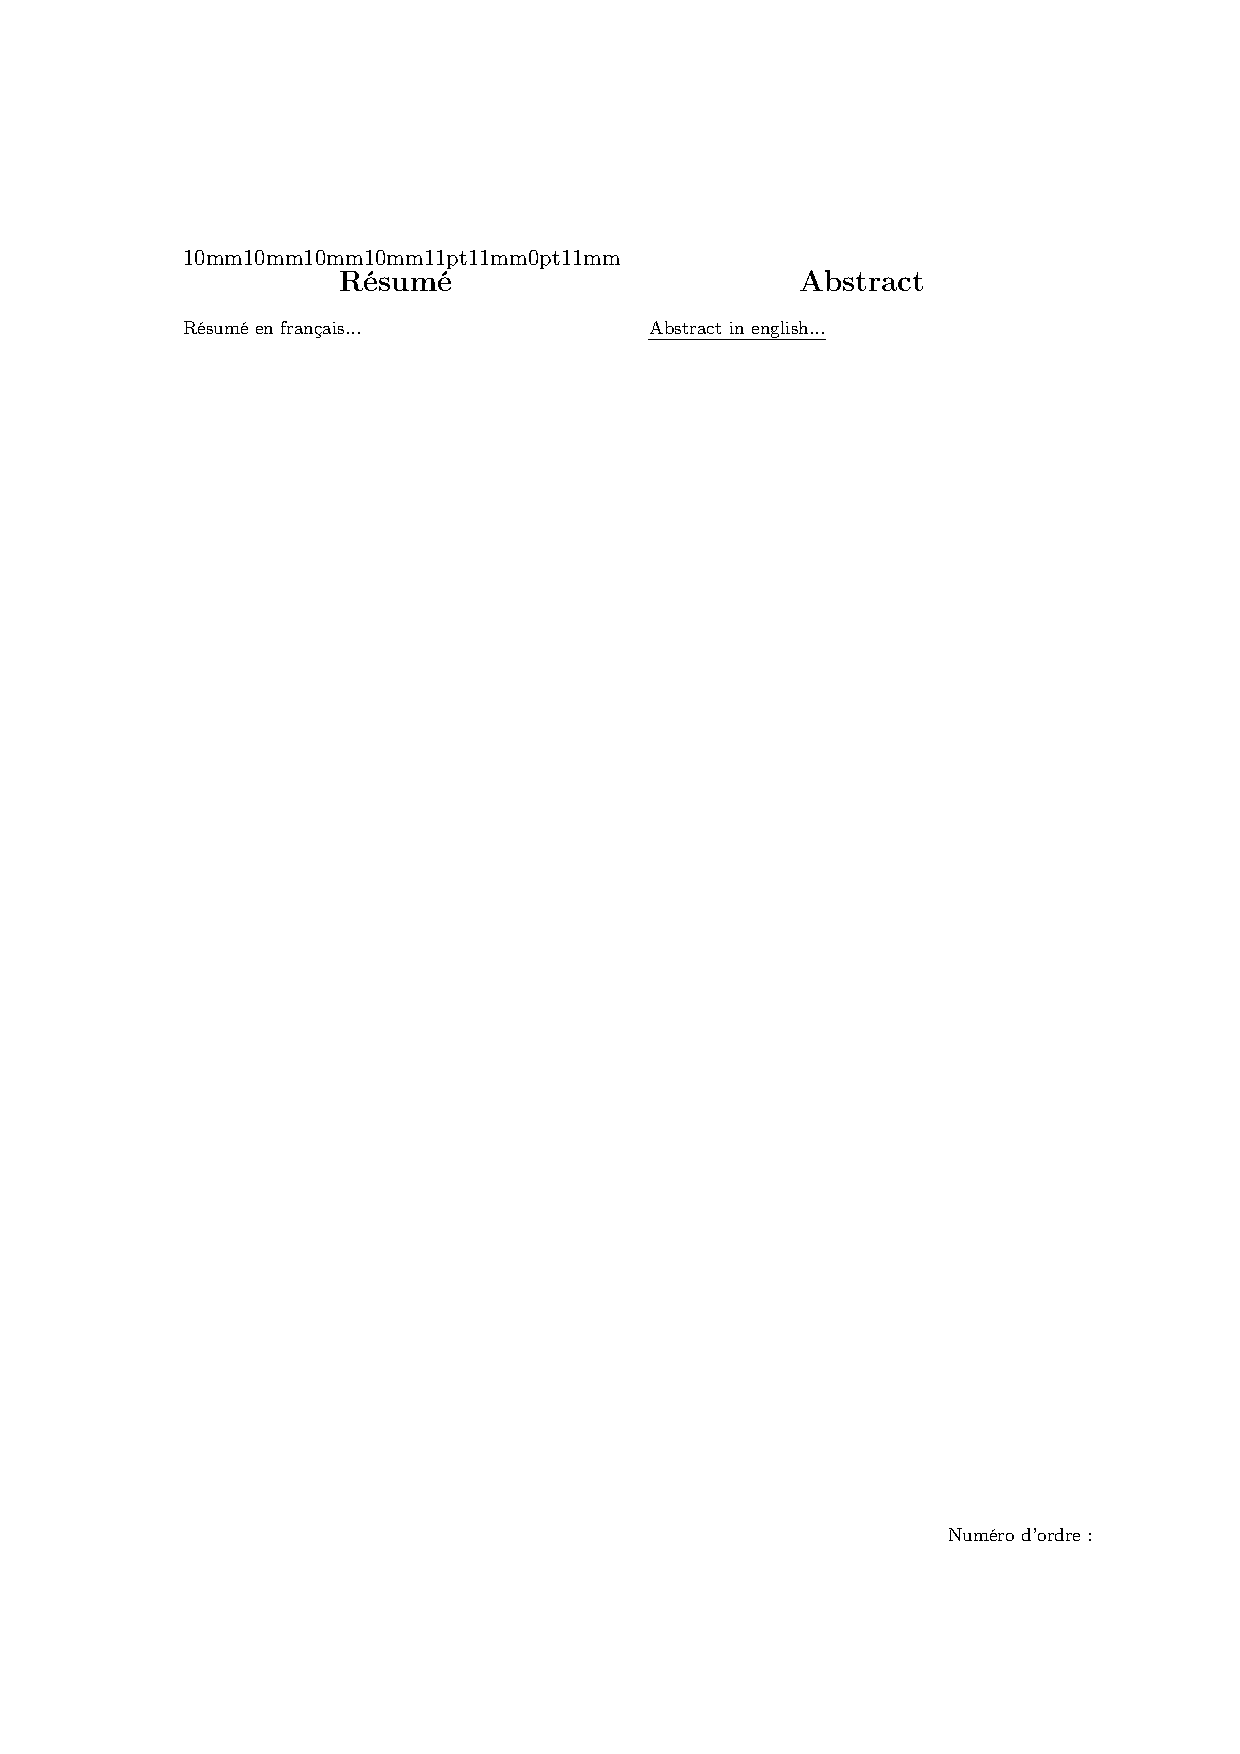
\includegraphics[width=\textwidth]{miscpages/resume.pdf}
\end{center}



\tableofcontents%%{Table des matières}
\markboth{Table des matières}{Table des matières}
\listoffigures%%{Liste des figures}
\markboth{Liste des figures}{Liste des figures}
\listoftables%%{Liste des tableaux}
\markboth{Liste des tableaux}{Liste des tableaux}
\printnomenclature%%{Liste des notations}
\markboth{Liste des notations}{Liste des notations}
\addcontentsline{toc}{chapter}{Liste des notations}
\mainmatter

% ------------------------------% ------------------------------%
\chapter*{Introduction Générale}
\addcontentsline{toc}{chapter}{Introduction générale}
\markboth{Introduction}{Introduction}
% ------------------------------% ------------------------------%



\glsresetall
\chapter{Contexte général de l'étude}

\section*{Introduction}
Ce stage resulte de plusieurs collaborations. D’une part elle result d’une collabo-
ration entre l’Université Nazi Bonin et L’université Lumière Lyon 2 dans le cadre du
programme erasmus+ mobilité etudiantes. C’est dans ce cadre que nous avons été
acceuillit au dans les locaux du LIRIS au sein de l’Université Lumière Lyon 2. Ce su-
jet de stage intitulé «segmentation géométrique et ghotométrique d’images acquises
par drones», resulte aussi d’une collaboration entre la société TECNI DRONE basée
à Baix (Ardèche) et l’equipe Imagine du LIRIS (site de l’Université Lumière Lyon
2 à Bron). TECNI DRONE se specialise dans la formation de pilot de drones et dans
l’acquisition de données géométriques issues de mines et de carrières. Les campagnes
d’acquisition d’images par drones, en milieu naturel, permettent de produire avec un
très haut niveau de qualité, des modèles numériques de terrains texturés, porteurs à
la fois d’informations géométriques et d’informations photométriques extrêmement
riches. De nombreuses recherches ont été menées au cours des dernières années, pour
affiner la qualité du traitement de ces données visuelles, et produire des maillages
texturés de plus en plus fiables. En revanche, l’exploitation de ces données reste pour
l’instant limitée soit à des traitements géométriques effectués sur les maillages 3D,
soit à des traitements d’images 2D, effectués par exemple sur les ortho-images obtenues 
par assemblage des multiples vues partielles.

\section{La structure d'accueil}

\subsection{Présentation }

 \subsubsection{Présentation du LIRIS}

Nous avons effectué notre stage au sein du Laboratoire d'InfoRmatique en 
Image et Systeme d'information \nomenclature{LIRIS}{Laboratoire d'InfoRmatique en Image et Systeme d'information}.
Le \nomenclature{LIRIS}{Laboratoire d'InfoRmatique en Image et Systeme d'information}est une unité miste de recherche  (\nomenclature{UMR}{Unité Mixte de Recherche} 5205) porté par
\begin{itemize}
  \item le CNRS
  \item l'INSA de Lyon
  \item l'Université Claude Bernard Lyon 1
  \item l'Université Lumière Lyon 2
  \item l'Ecole Centrale de Lyon
\end{itemize}
Il compte 330 membres, et a pour principal champ scientifique 
l'Informatique et plus généralement les Sciences et Technologies de l’Information.
Une partie importante de la recherche effectuée au LIRIS s’étend à la frontière de notre 
discipline, au service de problématiques sociétales importantes. Certaines des ses activités de 
recherche se situent aux interfaces de l’ingénierie, des sciences humaines et sociales, des sciences 
de la vie et des sciences de l’environnement. L’ensemble des 6 pôles de compétences du LIRIS participe 
de façon équilibrée à la valorisation des travaux de recherche. Par ailleurs, le LIRIS entretient de 
nombreuses relations avec son environnement social, économique et culturel, aussi bien aux niveaux 
local et régional qu’au niveau  national. 
Les interactions avec les entreprises s’établissent au travers de projets collaboratifs.
Le LIRIS couvre des thématiques scientifiques structurées en 6 pôles de compétences regroupant 14 équipes. 
\begin{itemize}
  \item Simulation, virtualité \& sciences computationnelles (Equipes Beagle, R3AM, SAARA)
  \item Géométrie \& modélisation (Equipes GeoMod, M2DisCo)
  \item Science des données (Equipes BD, DM2L, GOAL)
  \item Vision intelligente \& reconnaissance visuelle (Equipe Imagine)
  \item Interactions \& cognition (Equipes SICAL, SMA, TWEAK)
  \item Services, systèmes distribués, sécurité (Equipes DRIM, SOC)
\end{itemize}

Les travaux des équipes de recherche trouvent aussi des applications dans les secteurs : 
Biologie et santé (modelisation du vivant, ingénierie pour la santé), Intelligence ambiante 
(systèmes pervasifs et distribués, monitoring intelligent, systèmes autonomes), Apprentissage
humain (personnalisation, assistance cognitive, assistance à l'apprentissage collaboratif, 
jeux sérieux, loisirs numériques), Calcul scientifique (traitement de grandes masses de données
– big data).


\subsubsection{Presentation de l'equipe Imagine}
Nous avons effectués notre stage au sein de l'equipe Imagine sur le site de l'
université Lumière Lyon 2 à Bron.
L’équipe Imagine du LIRIS est spécialisée dans la vision par ordinateur, l’apprentissage 
et la reconnaissance de formes. Elle réunit 21 membres permanents (8 PR, 3 MCF-HDR et 10 MCF), 
enseignants-chercheurs de l’Université Lyon 1, de l’Université Lyon 2, de l’École Centrale de 
Lyon et de l’INSA Lyon.
En 2019, elle compte également parmi ses membres 29 doctorants et 17 post-doctorants.
Les différentes activités de recherche menées dans l’équipe Imagine partagent les mêmes 
objectifs généraux visant la compréhension d’images multi-sources et multi-capteurs, 
intégrant ainsi une très large variété de contenus autour des images de personnes, d’objets 
et de scènes en 2D et 3D (scènes naturelles ou urbaines, images aériennes et satellites, visages…), 
des séquences d’images et des flux vidéos, ainsi que des documents numérisés (cartes, textes écrits et 
imprimés, partitions et symboles…). La notion d’objet visuel, au sens large, constitue ainsi un 
dénominateur commun de nos recherches.
Les activités de l’équipe Imagine se déclinent en différentes thématiques 
liées à la mise en œuvre de méthodes d’indexation, de modélisation, 
de classification et de reconnaissance du contenu (objets, actions, concepts), 
avec une attention particulière portée au développement de méthodes d’apprentissage 
automatique pour la vision par ordinateur.
Les recherches menées dans l’équipe Imagine visent à construire des passerelles pour 
franchir le fossé sémantique entre, d’une part, les informations de bas niveau présentes 
dans les données brutes (données échantillonnées issues du signal), les éventuelles données 
multi-sources issues d’autres modalités ou capteurs (cas notamment des applications embarquées) 
et les informations de plus haut niveau sémantique qui reposent sur la modélisation, la 
classification et l’identification des contenus.
L’activité de recherche de l’équipe Imagine relève de 5 
sous-thèmes majeurs qui constituent le cœur de ses applications.

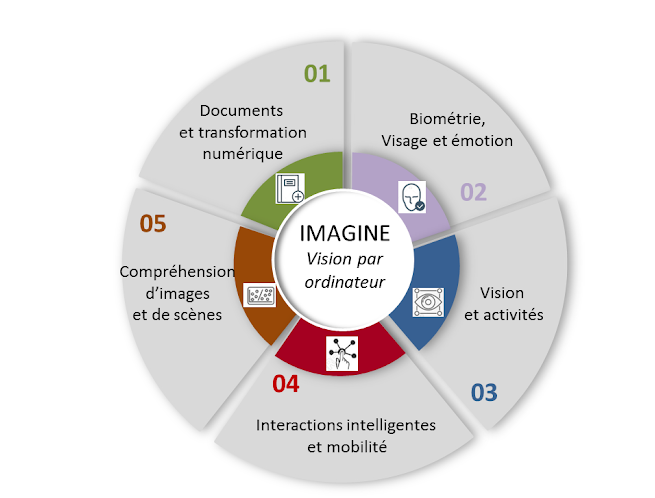
\includegraphics[scale=0.4]{images/Imagine.png}~\\[0.8cm]


 

  \subsection{Organisation}
   \subsubsection{Organigramme}  
L'organnigramme du LIRIS se présente comme suit: 
(voir Figure \ref{fig:organigramme}).
 \begin{figure}[h!]
  \begin{center}
    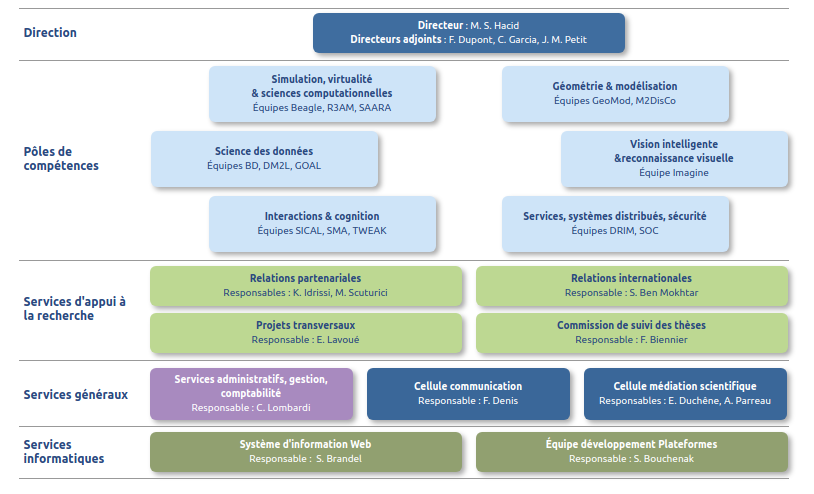
\includegraphics[width=17cm]{images/OrganigrammeLiris.png}
\caption{Organigramme du LIRIS.\label{fig:organigramme}}
\end{center}
\end{figure}


 \section{Présentation du sujet}

\subsection{Intitulé de sujet}

\textbf{Segmentation Géométrique etPhotométrique d’images Acquises par Drones}

 \subsection{Contexte du sujet}



\subsection{Intérêt du sujet}
 
Ce projet est très important pour Technidrone dans la mesure ou elle vise à
assister les techniciens de Technidrone dans leur tache d'annotation par la meme occasions reduire de façon 
significative le temps de travail de ces derniers.
Les résultats attendus sont:
\begin{itemize}
  \item Un gain en temps;
  \item Identification automatique des formes geometriques dans les images;
  \item 
\end{itemize}

    \subsection{Problématique du sujet}

    L’exploitation de données recoltées lors des campagnes d'acquisition reste pour
    l’instant limitée soit à des traitements géométriques effectués sur les maillages 3D,
    soit à des traitements d’images 2D, effectués par exemple sur les ortho-images obtenues
    par assemblage des multiples vues partielles. En revanche, la qualification de
    ces données, indispensable aux exploitants, reste pour l’instant un travail essentiellement manuel.
    Il s’agit par exemple, d’identifier les ruptures de pentes qui délimitent
    les voies de roulement des engins, de calculer la largeur de ces voies, de délimiter
    les hauts et les bas de talus, de calculer le volume des tas correspondant aux matériaux 
    extraits des carrières, etc. Ce processus qui est très important pour créer la
    carte d’une mine ou d’une carrière prend une dizaine d’heures pour un personnel
    entraîné. Une première etude effectuée au sein du laboratoire, axée essentiellement
    sur la geometrie contenue dans les maillages 3D a permis d’obtenir 62\% de rappel
    et 10\% de precision.

\subsection{Objectifs}

L’objectif de stage est d’utiliser d'une part les informations issues de la texture pour 
ameliorer les resultats obtenus en se basant uniquement sur la geometrie, et d'autre part, d’utiliser
de manière conjointe des informations issues des maillages, 
décrivant la géométrie de la scène, avec des données issues de la texture, portant des informations 
sur les discontinuités photométriques du terrain, pour assister les opérateurs dans leur tâche d’annotation 
des modèles numériques, construits à partir des images acquises par les drones.
En se basant sur des terrains déjà annotés, et en entraînant des classifieurs à reconnaître
les structures géométriques ou les motifs d’intérêt, nous voulons évaluer la capacité d’un système automatisé 
à effectuer cette identification avec un taux de succès le plus élevé possible. La tâche de 
l’opérateur se limiterait alors à la correction des inévitables erreurs de classification.

\section{Traitement des données et formats de fichiers}

TECHNI DRONE utilise plusieurs logiciels pour le traitement des donnéées après
les campagnes d'acquisition faites par drones. Cette etape est tres importante 
dans la mesure ou elle aboutie à la realisation des carte representant une carriere.

\begin{figure}[h]
  \begin{minipage}[c]{.46\linewidth}
      \centering
      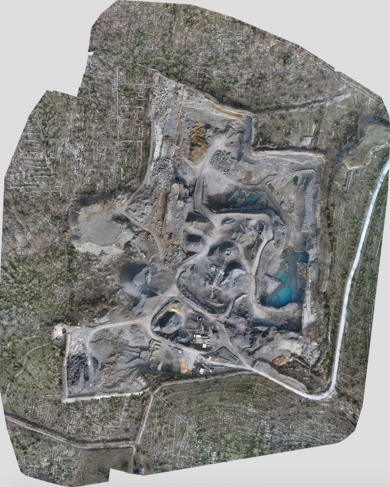
\includegraphics[width=8cm, height=8cm]{images/orthomosaique.png}
  \end{minipage}
  \hfill%
  \begin{minipage}[c]{.46\linewidth}
      \centering
      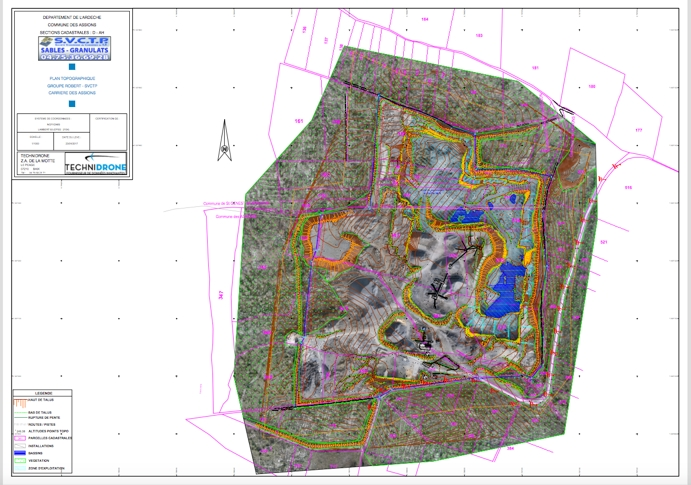
\includegraphics[width=8cm,height=8cm]{images/carteCarriere.jpg}
  \end{minipage}
  \caption{L’ortho mosaïque de la carrière et la carte de la carrière.
     \label{fig:credit}}
\end{figure}

\subsection{Pix4D}

Le traitement des images acquisent par drones est fait avec le logiciel Pix4D.
Pix4D est un logiciel de photogrammétrie pour la cartographie professionnelle 
basée sur des images de drones uniquement. 
\begin{figure}[h]
  \begin{center}
    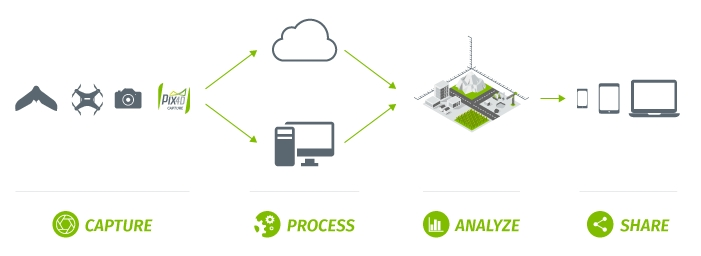
\includegraphics[width=12cm]{images/processusPix4D.jpg}
     \caption{Processus de traitement Pix4D.
     \label{ProcesPix4D}}
  \end{center}
\end{figure}
Le logiciel convertit les images 
aeriennes prise par drones en orthomosaiques 2D georeferencées, en model 
surface 3D texturé et en nuages de points. ce processus prend environ une dizaine
d'heures comment le montre la Figure~\ref{ProcesPix4D}. 

Dans la Figure~\ref{positionImage}, les points rouges representent les positions
des images prises drone et Les croix bleues sont les points GCPs
(Group Control Point)\footnote{Les GPCs sont des 
marqueurs visuels sur le sol avec des coordonnées connues qui augmentent 
la précision ortho mosaïque et permettent l'alignement de plusieurs 
campagnes d’acquisition.}. Le logiciel utilise les coordonnées des ces point
pour faire le recalage des images et produit les nuages de point et le maillage 3D
de la carrière. Le logiciel met aussi à disposition des outiles pour la detection
manuel des ligne de ruptures de pente directement sur les nuages de points ou
sur le maillage 3D. Les coordonnées de ces ligne ainsi detecter sont enregistrer
dans un fichier au format shapefile(.shp)\footnote{Shapefile est un format
de fichier ouvert compatible avec le logiciel OpenSource QGIS}. Cette phase
d'annotation prend egalement une dizaine d'heure pour un employé habitué au logiciel.
La Figure~\ref{annotationMallage} montre triangulaire 3D créé par pix4D,
sur lequel se basé pour détecter les lignes de ruptures de pente.

\begin{figure}[h]
  \begin{center}
    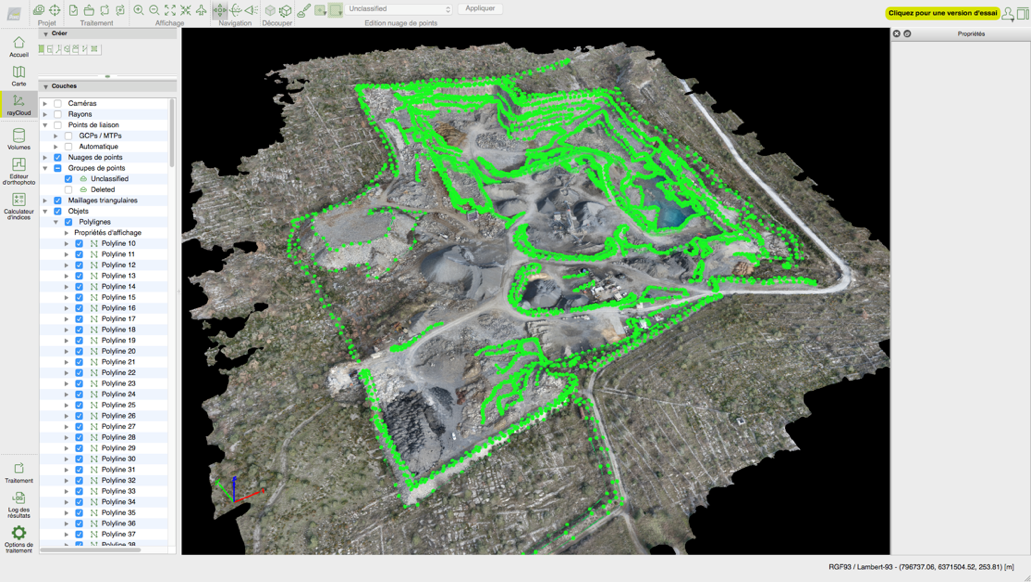
\includegraphics[width=12cm, height=5cm]{images/detctionLigne.jpg}
     \caption{Detection manuel des lignes de ruptures de pente.
     \label{detctionLigne}}
  \end{center}
\end{figure}
\begin{figure}[h]
  \begin{center}
    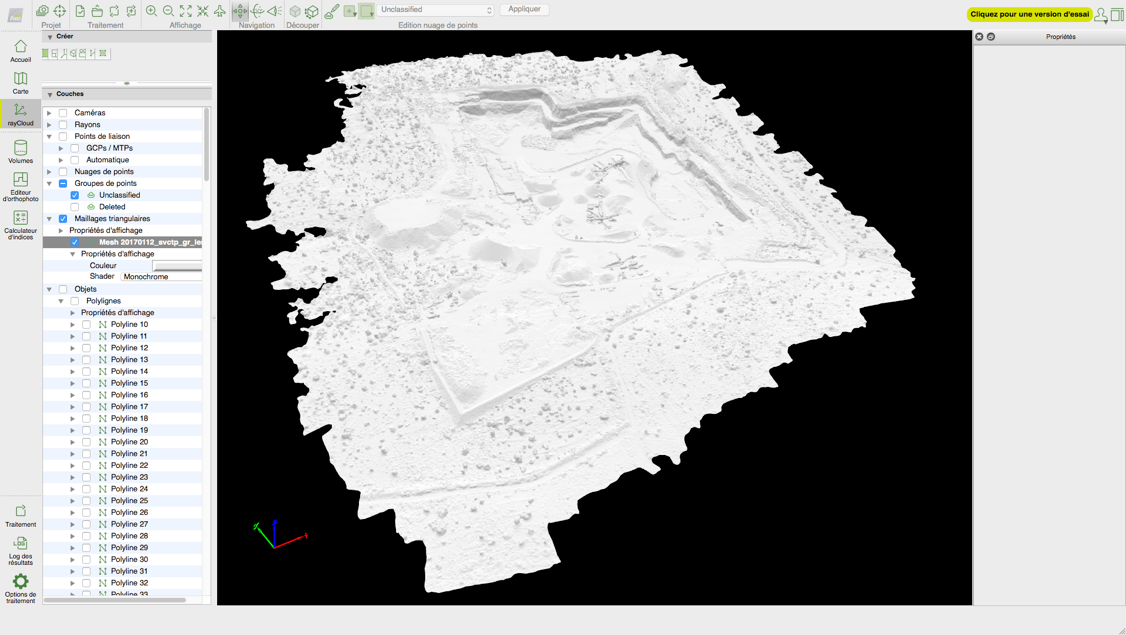
\includegraphics[width=12cm,height=5cm]{images/maillageSansTexture.jpg}
     \caption{Maillage 3D sans texture.
     \label{maillageSansTexture}}
  \end{center}
\end{figure}
\begin{figure}[h]
  \begin{center}
    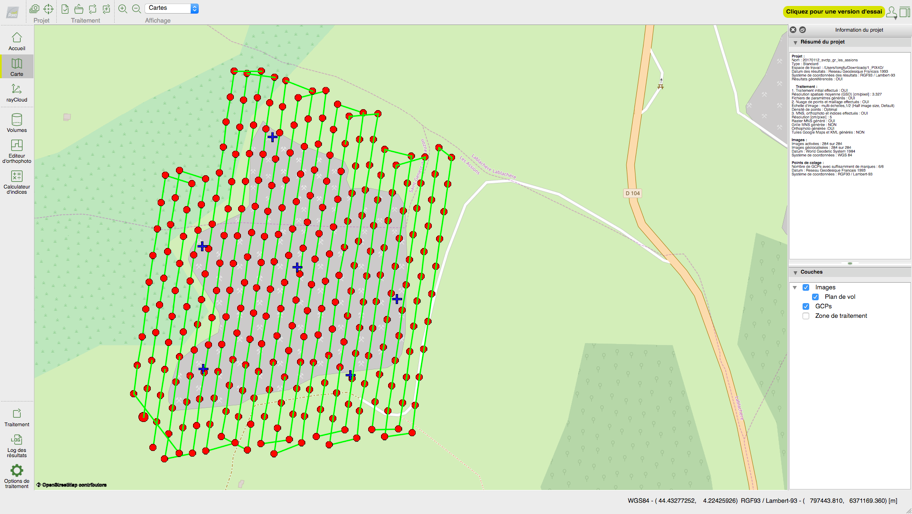
\includegraphics[width=12cm]{images/positionImagePix4D.jpg}
     \caption{Position des images prise par drones.
     \label{positionImage}}
  \end{center}
\end{figure}

\subsection{QGIS}

QGIS est un logiciel SIG (système d'information 
géographique) libre multiplate-forme publié sous licence GPL. 
il gère les formats d’image matricielles (raster) et vectorielles,
ainsi que les bases de données [Wikipedia](https://en.wikipedia.org/wiki/)\dots
TECHNI-DRONE utilise ce logiciel pour classifier les lignes de 
ruptures de pente par rapport aux courbes de niveau.
\begin{figure}[h]
  \begin{center}
    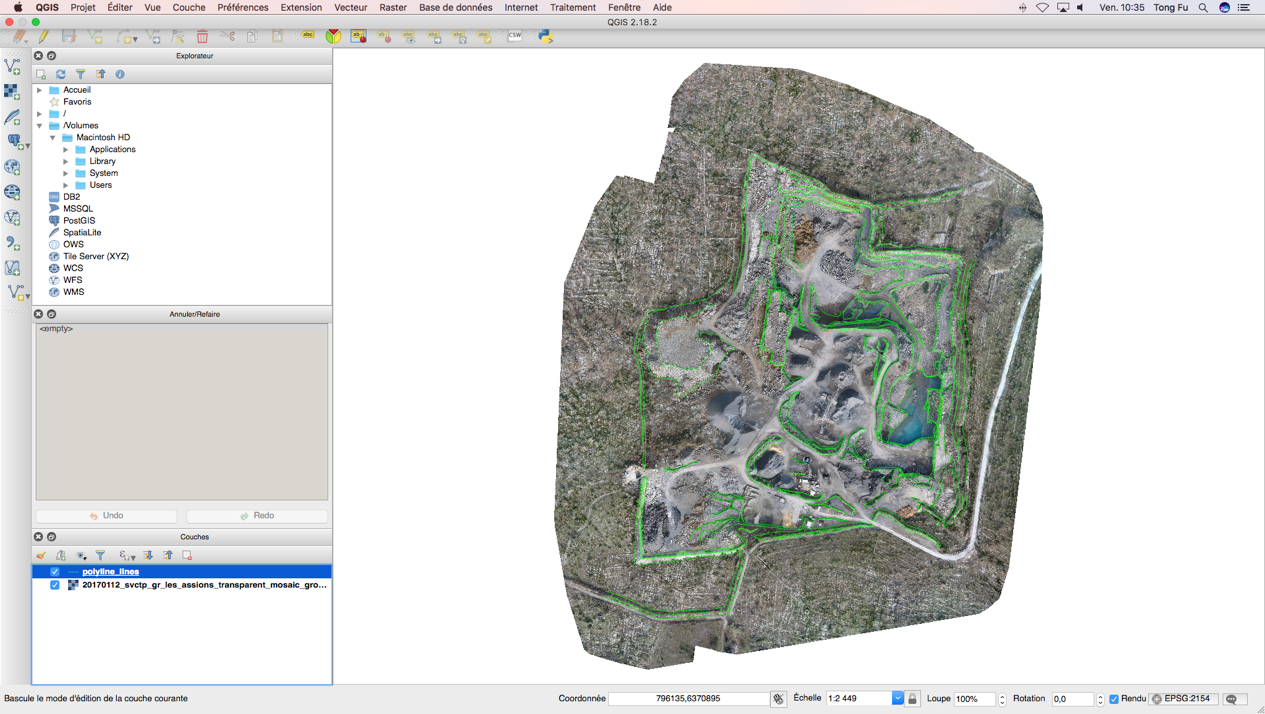
\includegraphics[width=12cm]{images/QGIS.jpg}
     \caption{Classification sur QGIS.
     \label{QGISClassification}}
  \end{center}
\end{figure}


\section*{Conclusion}
Dans ce chapitre il  a été question dans ce chapitre de présenter  la structure d’accueil,
au sein de laquelle nous avons menés nos travaux de recherche. .Ensuite nous avons
présenté le sujet qui qui fait objet de ce memoire, dégager sa problématique et
l’intérêt qu’il suscite pour la Société Technidrone. Dans le chapitre suivant,
nous parlerons des techniques machine learning, de la segmentation et de la classification.
 
\glsresetall
\chapter{Apprentissage automatique et aide à la décision}

\section*{Introduction}

Depuis plusieurs années, l'apprentissage automatique est de plus en plus exploré
en vue de résoudre des problèmes complexes pour lesquels les statistiques
étaient impuissante. L'objectif de l'apprentissage automatique (machine
learning) est de réaliser des modèles qui apprennent des exemples.
Le machine Learning est un ensemble de méthodes qui permettent aux ordinateurs
d'apprendre à partir des données qui leurs sont soumises. Historiquement,
cette théorie a pris son essor avec les travaux des mathématiciens Vapnik et
Chervonenkis dans les années 60. Avec le Machine Learning, le point de vue est
différent de celui de la statistique traditionnelle. Les algorithmes d'apprentissage
automatique permettent aux ordinateurs de s'entraîner sur les entrées de données et 
utilisent l'analyse statistique pour produire des valeurs qui se situent dans une 
plage spécifique.


\section{Vocabulaire du machine learning}

\subsection{Etiquettes}
Une étiquette est le résultat de la prédiction ; la variable y dans une régression 
linéaire simple. Il peut s'agir du cours à venir du blé, de l'espèce animale représentée 
sur une photo ou de toute autre chose. 
Dans l'analyse d'un dossier, les étiquettes sont le résultat de l'analyse d'un
dossier.

\subsection{Caractéristiques}
Une caractéristique est une variable d'entrée ; la variable x dans une régression linéaire 
simple. Un projet de Machine Learning simple peut utiliser une seule caractéristique, 
tandis qu'un projet plus sophistiqué en utilisera plusieurs, spécifiées sous la forme :
$$
x1, x2, \ldots{}, x3
$$
\subsection{Exemples}
Un exemple est une instance de donnée particulière, x. Les exemples se répartissent dans deux
catégories : les exemples étiquetés et les exemples non-étiquetés.

\subsection{Modèles}
Un modèle définit la relation entre les caractéristiques$X$ et l'étiquette.
Par exemple, un modèle de détection de spam peut associer étroitement certaines
caractéristiques à du \og spam \fg.

Les principales étapes de la durée de vie d'un modèle sont les suivants:
\subsubsection{L'apprentissage}
L'apprentissage consiste à entraîner le modèle. En d'autres termes, il s'agit de
présenter au modèle des exemples étiquettés et de lui permettre d'apprendre
progressivement les relations entre les caractéristiques et l'étiquette.

\subsubsection{L'inférence}

L'inférence consiste à appliquer le modèle entraîné à des exemples sans
étiquette. Il s'agit  d'utiliser le modèle entrainé pour faire des prédictions
efficace.



%\input{sources/chapter3_ml/etape.tex}

\section{Les objectifs et méthodes du Machine learning}

Le choix de la méthode d'apprentissage dépend en grande partie de l'objectif
poursuivi.

\subsection{Les objectifs du machine learning}

Le machine learning poursuit plusieurs objectifs qui selon le cas peut être
 \subsubsection{Une classification}
Les modèles de classification prédisent des valeurs discrètes. Ils formulent, 
par exemple, des prédictions qui répondent à des questions telles que les suivantes:
\begin{itemize}
  \item Un e-mail donné est-il considéré comme du spam ou non?
  \item Cette image représente-t-elle un chien, un chat ou un hamster?
  \item Un dossier donné est-il conforme ou pas?
\end{itemize}

La classification est un processus en deux étapes, une étape 
d’apprentissage et une étape de prédiction, dans l’apprentissage machine.
Dans l’étape d’apprentissage, un modèle est développé à partir d’un 
ensemble de données préalablement étiquettés. Dans la phase de prédiction,
le modèle développé dans la phase précédente est utilisé pour prédire les 
étiquettes de nouvelles données.

\subsubsection{Une regression}
Les modèles de régression prédisent des valeurs continues. Ils formulent,
par exemple, des prédictions qui répondent à des questions telles que :
\begin{itemize}
  \item Quel est la valeur d'un logement au Burkina Faso ?
  \item Quel est la probabilité qu'un utilisateur clique sur cette annonce?
\end{itemize}

\subsubsection{Le clustering}
Le clustering est le regroupement d'exemples en classes d'objets similaires.
La différence entre clustering et classification est que les exemples sont
étiquetés dans une classification alors que dans le clustering, il ne le sont
pas.(Voir Figure \ref{fig:clustering})


\begin{figure}[h!]
  \begin{center}
    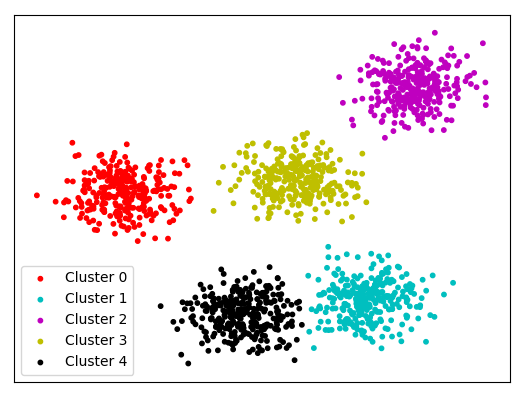
\includegraphics[width=14cm]{images/clustering.png}
      \caption{Clustering des données.\label{fig:clustering}}
  \end{center}
\end{figure}

Le but des algorithmes de clustering est de donner un sens aux données et
d'extraire de la valeur à partir de grandes quantités de données structurées ou
non-structurées. Ces algorithmes vont permettre de séparer les données en
fonction de leurs propriétés ou fonctionnalités et de les regrouper dans
différents clusters en fonction de leurs similitudes.




\subsection{Les méthodes d'aprentissage}
Les méthodes d'apprentissage automatique les
plus largement adoptées sont l'apprentissage supervisé et l'apprentissage
non-supervisé. Explorons donc ces méthodes plus en détail.

\subsubsection{L'apprentissage supervisé}
Le but de cette méthode est de permettre à l'algorithme  de découvrir 
l'étiquette réelle d'un exemple à partir des étiquettes apprises pendant la
phase d'entrainement, pour trouver des erreurs et modifier le modèle en 
conséquence. L'apprentissage supervisé utilise pour l'entrainement de son modèle,
des exemples étiquettés.

\subsubsection{L'apprentissage non-supervisé}
L’apprentissage non supervisé consiste à apprendre à classer sans supervision; les
exemples fournis sont non-étiquettés. L'objectif ici  est de réunir les 
exemples selon des critères prédéfinis par les équipes en charge du projet.En effet,
l’apprentissage non supervisé permet de regrouper des éléments non-classés dans 
différents groupes selon leurs caractéristiques.


\section{Les différents type de classifieurs}

Il existe plusieurs types de classifieurs. Nous présentons içi quelques
classifieurs avec leurs avantages et inconvénients.

 \subsection{Méthode des K plus proche voisins (KNN)}

La méthode des 'K plus proche voisins' ou \textbf{k-Nearest Neighbors
KNN} en \nomenclature{KNN}{K-Nearest Neighbors}
anglais est une méthode de classification dans laquelle le modèle mémorise 
les observations de l’ensemble d’apprentissage pour la classification des 
données de l’ensemble de test.\cite{pradaig}

Son fonctionnement peut être assimilé à l’analogie suivante:
\textit{dis moi qui sont tes voisins, je te dirais qui tu es}.
Pour effectuer une prédiction, l’algorithme \textbf{K-NN} ne va pas calculer
un modèle prédictif à partir d’un training set(ensemble d'apprentissage) comme c’est le cas pour la 
régression logistique ou la régression linéaire. C'est pourquoi cet 
algorithme est qualifié de paresseux (Lazy Learning) car il n’apprend
rien pendant la phase d’entrainement. 

\subsubsection{Prédiction avec K-NN}
K-NN se base sur le jeu de donnée entier pour effectuer une prédiction. Pour 
un exemple qu'on souhaite prédire qui ne fait pas parti du jeu de données \cite{datascientist}
initiale, l’algorithme va chercher les \textit{K} instances du jeu de données les 
plus proches de notre exemple. Ensuite pour ces \textit{K} voisins, l'algorithme
se basera sur leurs étiquettes pour calculer l'étiquette de l'exemple que l'on
souhaite prédire.(figure~\ref{fig:knnfonctionnement})

\subsubsection{Similarité dans l'algorithme K-NN}
K-NN a besoin d’une fonction de calcul de distance entre deux exemples. Plus 
deux points sont proches l’un de l’autre, plus ils sont similaires et vice 
versa\cite{nagesh2019}.

Il existe plusieurs fonctions de calcul de distance, notamment, la distance 
euclidienne, la distance de Manhattan, la distance de Minkowski, celle de 
Jaccard, la distance de Hamming \ldots. La fonction de distance se choisit en
fonction des types de données qu’on manipule. Ainsi pour des données 
quantitatives (poids, salaires, taille, montant de panier éléctronique\ldots),
la distance euclidienne est un bon candidat. Quant à la distance de Manhattan,
elle est une bonne mesure quand les données ne sont pas de 
même type (age, sexe, longueur, poids\ldots).

\begin{figure}[h!]
  \begin{center}
    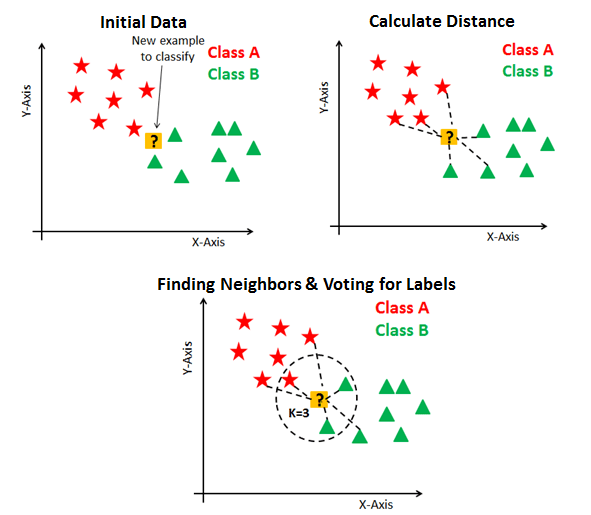
\includegraphics[width=12cm]{images/knn.png}
    \caption{Fonctionnement de l'algorithme K-NN.\label{fig:knnfonctionnement}}
  \end{center}
\end{figure}

\subsubsection{Choix de la valeur K}

Le choix de la valeur K varie en fonction du jeu de données. En règle générale, 
si K est petit, on sera sujet au sous apprentissage (underfitting). Par 
ailleurs, plus on utilise de voisins (K grand) la prédiction sera plus fiable. 
Toutefois, si on utilise K nombre de voisins avec K=N et N étant le nombre 
d’exemples, on risque d’avoir du overfitting et par conséquent un modèle qui se
généralise mal sur des observations qu’il n’a pas encore vu.

\subsubsection{Avantages}
\begin{description}
     \item{\textit{Absence d'apprentissage}}: Ce sont les échantillons pris en 
      considération, qui constituent le modèle.
    \item{\textit{Clarté des résultats: }} bien que la méthode ne produise pas de 
        règle explicite, la classe attribuée à un exemple peut être expliquée en
        exposant les plus proches voisins qui ont imposé cette attribution.
       \item{\textit{Grand nombre d'attributs:}} la méthode permet de traiter des
          problèmes avec un grand nombre d'attributs. Cependant, plus le nombre 
          d'attributs est important, plus le nombre d'exemples doit être grand.
      \end{description}

\subsubsection{Inconvénients}
\begin{description}
   \item{\textit{Sélection des attributs pertinents:}} Pour que la notion de proximité
    soit pertinente, il faut que les exemples couvrent bien l'espace et soient 
    suffisamment proches les uns des autres. Si le nombre d'attributs pertinents est
    faible relativement au nombre total d'attributs, la méthode donnera de mauvais 
    résultats.
   \item{\textit{Le temps de classification:}} Si la méthode ne nécessite pas 
    d'apprentissage, tous les calculs doivent être effectués lors de la classification 
    d'un nouvel exemple.
  \item{\textit{Définir les distances et nombres de voisins:}} Les performances de la 
      méthode dépendent du choix de la distance, du nombre de voisins et du mode de 
      combinaison des réponses des voisins.
  \end{description}

\subsection{Les réseaux de neurones}
Les réseaux de neurones sont inspirés de la structure neurophysiologique des
neurones. En règle générale, un réseau de neurones repose sur un grand nombre de
processeurs opérant en parallèle et organisés en tiers(couches). La première
couche reçoit les entrées d’informations brutes, un peu comme les nerfs optiques
de l’être humain lorsqu’il traite des signaux visuels. Par la suite, chaque
couche  reçoit les résultats de la couche précédente.
On retrouve le même processus chez l’Homme, lorsque les neurones reçoivent des
signaux en provenance des neurones proches du nerf optique. La dernière couche,
quant à elle, produit les résultats du système.

\subsubsection{Les différents cas d'usage}

Les réseaux de neurones sont beaucoup utilisés dans la reconnaissance d'écriture
manuscrites, la transcription \og speech-to-text \fg ou encore dans la
prévision des marchés financiers ou trading algorithmique.

Ils peuvent aussi être utilisé pour la reconnaissance faciale, la prédiction
météo, la détection de cancer sur les imageries médicales. De manière générale,
les réseaux de neurones excellent pour la reconnaissance de patterns.

\subsubsection{Avantages}
\begin{description}
  \item{\textit{Classification efficace :}} le calcul d'une sortie à partir d'un 
    vecteur d'entrée est un calcul très rapide.
  \item{\textit{Les données réelles :}} les réseaux traitent facilement les données 
      réelles "préalablement normalisées" et les algorithmes sont robustes au bruit.
  \end{description}

\subsubsection{Inconvénients}
\begin{itemize}
  \item Déterminer l’architecture du réseau est complexe et les
    paramètres sont difficiles à interpréter (boite noire).
    \item L'échantillon nécessaire à l'apprentissage doit être
      suffisamment grand et représentatif des sorties attendues.
  \end{itemize}

\subsection{Support Vector Machine (SVM)}
Les Support Vector Machine ou Machine à Vecteur de Support constituent une 
technique d’apprentissage supervisée. Elles ont été inventées par Boser, 
Guyon et Vapnik \cite{10.1145/130385.130401} et présentées pour la première
fois à la conférence Computational Learning Theory (COLT) de 1992.
Grâce à ses performances \cite{Cortes1995}, cette technique a ouvert un domaine de 
recherche très actif et un grand éventail d’applications. Les SVM utilisent
une approche géométrique pour classer les données en deux catégories.

En considérant les données comme des vecteurs, les SVM construisent un plan(une
frontière) qui sépare les données dans chacune des catégories.
Une fois la frontière de décision construite(Hyperplan) la
SVM\nomenclature{SVM}{Support Vector Machine} sera capable de
classer de nouvelles données en observant de quel côté de la frontière elles
tombent, et en leur assignant la catégorie correspondante.

L'idée est donc de rechercher le meilleur hyperplan qui sépare linéairement deux
classes, tout en les repoussant aux maximum. Lors de la phase d'apprentissage,
le svm cherche à maximiser la marge entre les deux classes d'apprentissage. Ce
qui lui procure une grande capacité de généralisation pendant la phase de test.

Les machines à vecteurs de support ont été appliquées dans des domaines comme
la reconnaissance automatique des visages et des gestes \cite{840634}, la
prédiction des mouvement de la bourse\ldots \cite{HUANG20052513}.

 Les domaines dans lesquels, elles sont les plus efficace sont: la reconnaissane d'objet et de
 d'image \cite{788125} et la catégorisation de texte \cite{6990940}



\begin{figure}[h!]
  \begin{center}
    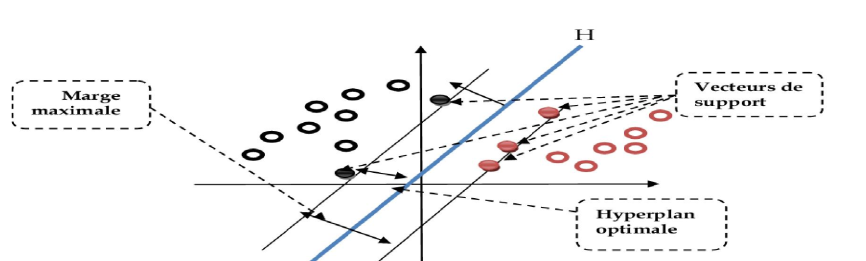
\includegraphics[width=14cm]{images/marge.png}
      \caption{Machine à vecteurs de support .\label{fig:marge}}
  \end{center}
\end{figure}

\subsubsection{Avantage}
\begin{itemize}
  \item Grâce à leurs fondements mathématiques solides, les SVM possèdent donc
    une grande précision de prédiction
  \item les SVM fonctionnent bien sur de petits jeux de données
  \item Décision rapide. La classification d’un nouvel exemple consiste à voir le signe de
    la fonction de décision f(x). 
\end{itemize}

\subsubsection{Inconvénient}
Les SVM ne conviennent pas à des jeux de données très volumineux car le temps
d'entrainement est très long.

  Les SVM effectuent une classification binaire d’où la nécessité d’utiliser 
l’approche un-contre-un pour construire un classifieur multiclasse.
Une grande quantité d’exemples en entrées implique un calcul matriciel important.
Le temps de calcul est élevé lors d’une régularisation des paramètres de la 
fonction noyau. 

Les SVM sont moins efficaces sur les jeux de données contenant
du bruits et beaucoup d’outliers

 \subsection{Les arbres de décisions}
Un arbre de décision est un outil d’aide à la décision qui permet de
répartir une population d’individus en groupes homogènes selon des attributs
discriminants en fonction d’un objectif fixé. Il permet d'émettre des
prédictions sur le problème par réduction niveau après niveau du domaine.

Les arbres de décision sont facilement interprétables, toutefois, leur capacité de
prédiction est presque toujours dépassée par les autres modèles de classication. 
Cette caractéristique a limité son utilisation. Au début des années 2000,
ils ont été repris comme élément de base d'une nouvelle méthode de
classification, appelée la forêt aléatoire de décision.

Cette nouvelle technique utilise de manière combinée les arbres de
décision et la théorie statistique pour réduire la variance du classeur en calculant la
moyenne d'un ensemble d'arbres de décision en générant des classeurs avec une très
bonne capacité de prévision. Nous les présenterons plus largement dans les
prochaines sections.

\subsubsection{Avantages}
\begin{description}
   \item{\textit{Adaptabilité aux attributs de valeurs manquantes :}} les
    algorithmes peuvent traiter les valeurs manquantes (exemples contenant
    des champs non renseignés) pour l'apprentissage, mais aussi pour la 
    classification.
  \item{\textit{Modèle white-box }} D'un arbre de décision, il
    est possible de générer des règles permettant d'expliquer ou de comprendre le
    résultat d'une classification. le résultat est facile à conceptualiser, 
    à visualiser et a interpréter.
  \item{\textit{Classification très rapide :}} Le coût d'utilisation des arbres est
    logarithmique.
  \item{\textit{Traitement de tous type de données: }} Les arbres de décisions
    prennent en compte aussi bien les échantillons ayant des caractéristiques
    continues que discrètes. Il est robuste au brruit.
  \item{\textit{Donne une classification efficace}} L'attribution d'une classe à
    l'aide d'un arbre de décision est obtenu grâce au parcours d'un chemin de
    l'arbre.
  \item{\textit{Ils ont un bon comportement par rapport aux valeurs extrêmes
    (outliers).}}
\end{description}

\subsubsection{Inconvénient}
  \begin{description}
     \item{\textit{Manque d’évolutivité dans le temps :}} Même si les données
      évoluent avec le temps, il est nécessaire de relancer une phase d'apprentissage 
      sur l'échantillon complet (anciens nouveaux exemples)
     \item{\textit{Méthode sensible au nombre de classes :}} les performances tendent à
      se dégrader lorsque le nombre de classes devient trop important.
    \item{\textit{Ils sont instables :}} D es changements légers dans les données produisent des 
      arbres très différents. Les changements des nœuds proches de la racine affectent 
      beaucoup l’arbre résultant. 
    \item{\textit{Sûr-apprentissage :}} Les arbres générés sont trop complexes et généralisent 
      mal (solution : élagage, contrôle de la profondeur de l’arbre et de la taille 
      des feuilles).
  \end{description}




\section{Comparaison des algorithmes de classification}

Le choix de l'algorithme optimal pour un problème donnée dépend de sa vitesse
d'entrainement et de prédiction, de la précision de ces prévisions, de la
quantité de données nécessaires à l'entrainement, de la facilité à la mettre en
oeuvre, et de la capacité à expliquer le résultat de la prédiction.

Le tableau ci-dessous présente une comparaison des différents algorithmes de
classification.

\begin{table}
  \begin{center}
    \renewcommand{\arraystretch}{1.5}

    \begin{tabular}{|c|c|c|c|c|c|}
      \hline
      \rowcolor[gray]{0.7}
      \bf\rule[-0.4cm]{0mm}{1cm} Algo & \bf Interprétabilite & \bf Précision & \bf{VE et VP} & \bf Données \\
      \hline
     \bf Knn & Oui & Faible & Dépend de K & Beaucoup \\
      \hline
     \bf Régression & Un peu & Faible & Rapide & Peu \\
      \hline
     \bf Naïves bayes & Un peu & Faible & Rapide & Peu \\
      \hline
     \bf Réseaux de neurones & non & Très élevé & Lent & Beaucoup \\
      \hline
      \bf{Arbre de décision} & Oui & Moyen & Rapide & Assez \\
      \hline
      \bf{Random Forest} & Non & Très élevé & Lent & Assez \\
      \hline
    \end{tabular}
    \caption{Tableau de comparaison des algorithmes de classifications}
    \label{tab:tab2}
  \end{center}
\end{table}
Le tableau \ref{tab:tab2} révèle que les algorithmes de Réseaux de neurones et ceux de forêt
aléatoire ont un taux très élevé de bonne prédiction. Malheureusement, ces
algorithmes fonctionnent bien sur des jeude données énormes. De plus la vitesse
d'apprentissage et de prédiction reste relativement lente par rapport aux
autres algorithmes.



\section{Les arbres de décisions}

Deux techniques de classification par les arbres ont été dévéloppées au
début des années 1980 par deux groupes de chercheurs.
Le premier groupe, dirigé par J Ross Quinlan, a développé un algorithme d'arbres
de décision en 1986 appelé ID3. Plus tard en améliorant plusieurs 
caractéristiques de ID3, il a développé et présenté C4.5.
L. Breiman, J. Friedman, R. Olshen, et C. Stone, un groupe de statisticiens, 
ont développé un algorithme pour produire des arbres de décision binaires 
appelé CART (Classication and Regression Trees) de leur côté. Ces algorithmes
ont été le début de la recherche sur la classification par les arbres de
décisions.  Les deux approches suivent le paradigme \og Diviser pour régner \fg

Plusieurs objectifs concourent à la construction d'un arbre de décision. Ce
sont:
\begin{itemize}
  \item Une meilleure généralisation des exemples de la base d'apprentissage.
  \item Une meilleure classification de nouveaux exemples
  \item Une structure aussi simple que possible
\end{itemize}
La construction d'un arbre de décision consiste à partitionner un ensemble de 
données en des groupes les plus homogènes possible du point de vue de la 
variable à prédire. On prend en entrée un ensemble de données classées, et on 
fournit en sortie un arbre. Nous obtenons un arbre qui représente une série de 
noeuds en plaçant dans la partie supérieure le noeud dont la capacité de 
classification est la plus grande. \cite{criminisi2011} 
Le résultat final est un arbre renversé comme celui représenté dans la figure
\ref{fig:DecisionTree}

\begin{figure}[h!]
  \begin{center}
    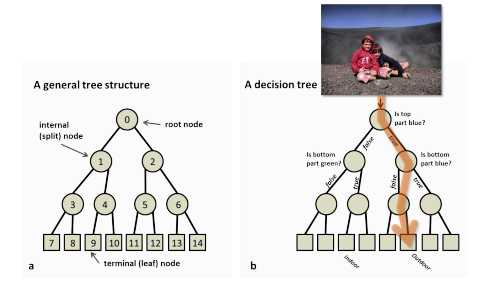
\includegraphics[width=14cm]{images/decisionTree.png}
    \caption{Arbre de décision. 
	\label{fig:DecisionTree}}
  \end{center}
  \textit{Le $a$ représente la structure générale d'un arbre de décision. Le
$b$ montre un arbre de décision illustratif utilisé pour déterminer 
si une photo représente une scène d'intérieur ou d'extérieur.}
\end{figure}

\subsection{Structure d'un arbre de décision}

Le fonctionnement des arbres de décisions repose sur les heuristiques 
construites sur des techniques d'apprentissage supervisées.

Les arbres de décisions sont composés de noeuds et de feuilles reliés par des
branches. Dans leur représentation graphique la raçine est placée tout en haut
et les feuilles en bas. Les noeuds internes sont appelés des noeuds de décision.
Ils peuvent contenir une ou plusieurs règles. Les noeuds terminaux contiennent
la classe aussi appelée classe à prédire ou étiquette. Après sa construction, un
arbre de décision peut être traduit par un ensemble de règle.

L'algorithme  générique  de construction d'un arbre permet de générer
itérativement l'arbre en prenant à chaque itération une variable et en lui
créant ses noeuds et ses feuilles. L'idée centrale est la suivante:

\textit{Diviser récursivement et le plus efficacement possible les exemples de  
l'ensemble d'apprentissage par des tests définis à l'aide des attributs
jusqu'à ce que l'on obtienne des sous-ensembles d'exemples ne contenant 
(presque) que des exemples ayant tous la même étiquette.}

 \subsection{Optimisation des noeuds}
 
 En général, on décide qu'un noeud est terminal lorsque tous les exemples
 associés à ce noeud, ou du moins  la plupart d'entre eux ont la même étiquette
 ou s'il n'y a plus d'autres caractéristiques non utilisées dans la branche
 correspondante.

 La sélection d'un test à associer à un noeud pour obtenir un arbre optimal 
 est un choix crucial. En effet, construire un arbre de décision optimal
 consiste à construire un arbre de décision le plus petit possible rendant compte
 au mieux des données. Il s'agit donc de rechercher le test qui permet de faire
 évoluer la tâche de classification. Pour mesurer cette évolution, \textit{CART}
 utilise l'\textit{indice de Gini}. Les algorithmes de Quinlan eux, utilisent  la
 notion d'\textit{entropie}.

 \subsubsection{Entropie de Shannon}

L'entropie de Shannnon correspond à la quantité d'information fournies par un
évènement: plus la probabilité d’un événement est faible (il est rare), plus 
la quantité d’information qu’il apporte est grande. Sa formule est la
suivante
\cite{benjamin2005}:
$$  
Entropie = - \sum_{i=1}^{n} {p_i * log_2(p_i)}
$$ 
Tel que $p_i$ est la proportion d'exemples de S ayant pour classe résultante
(étiquette) $i$. 

Pour un ensemble de données $T$ caractérisé par $n$ classes ($C_1, C_2, \cdots,
C_n$) selon la variable cible, la quantité d'information nécessaire pour
identifier la classe d'un individu correspond à l'entropie $E(P)$ où $P$est la
distribution de probabilité de la partition ($C_1, C_2, \cdots, C_n$).
$$
P = (\frac{|C_1|}{|T|}, \frac{|C_2|}{|T|}, \cdots, \frac{|C_n|}{|T|})
$$
$|C_i|$ représente le cardinal de la classe $i$ c'est-à-dire le nombre
d'éléments de la classe $i$.

L'entropie de $T$ est alors:

$$
Entropie(T) = - \sum_{i=1}^{n}{\frac{|C_i|}{|T|} log_2\frac{|C_i|}{|T|}}
$$

La fonction permettant de sélectionner le test qui doit étiqueter le noeud
courant  est la fonction \textit{Gain}. Pour un ensemble de données $T$, le gain
d'information de $T$ par rapport à une partition $T_j$ donnée est la variation
d'entropie causée par la partition de T selon $T_j$
$$
Gain(X, T) = Entropie(T) - Entropie(X, T) = Entropie(T) - \sum_{j=1}^{m} {\frac{T_j}{T} * Entropie(T_j)}
$$

Le gain permet de calculer ce que l'attribut spécifié apporte au désordre
du set. Plus un attribut contribue au désordre, plus il est important de le
tester pour séparer le set en plus petits sets ayant une entropie moins 
élevée.

\subsubsection{Indice de Gini}
L'indice de Gini est une mesure statistique permettant de rendre compte de la
répartition d'une variable au sein d'une population. Il mesure l'impureté qui
est un concept très utile dans la construction des arbres de décision: La qualité
d'un noeud et son pouvoir discriminant peuvent être évalués par son impureté.
Sa formule est la suivante:
$$
Gini(T) = 1 - \sum_{j=1}^{m}{(p_i)^2} =  1 - \sum_{j=1}^{m}{(\frac{|T_j|}{|T|})^2} 
$$




\subsection{Algorithmes d’induction d’arbres de décision}

Il existe essentiellement deux grandes familles d'algorithmes permettant de construire
des arbres de  décisions à partir d'un set de données: les algorithmes de
Quinlan (\textbf{ID3}, \textbf{C4.5}, \textbf{C5.0}) et l'algorithme
\textbf{CART}. Les deux approches suivent le paradigme \og diviser pour régner
\fg. Nous présentons ici le principe des trois algorithmes de construction des
arbres de décision que sont l'algorithme ID3, l'algorithme C4.5 et l'algorithme
CART.

%\input{sources/chapter4_arbre/generic}

   \subsubsection{CART}
  L'algorithme Classification and Regression Trees(\textit{CART}) est très
  similaire à C4.5, mais il en diffère par le fait qu’il prend en charge la
  régression en ne calculant pas des ensembles de règles. Il s'agit d'un  
  algorithme développé par Breiman, Friedman, Olshen et Stone (1984).

  Selon l'algorithme CART, un arbre de décision est construit en déterminant
  les questions (appelées fractionnements de noeuds) qui, lorsqu'on y répond,
  conduisent à la plus grande réduction de l'impureté de Gini. Cela signifie 
  que l'arbre de décision tente de former des noeuds contenant une forte 
  proportion d'échantillons (points de données) provenant d'une seule classe en
  trouvant des valeurs dans les caractéristiques qui divisent proprement les 
  données en classes(étiquettes).
 
  \subsubsection{ID3}
  Iterative Dichotomiser 3(\textit{ID3}) a été developpé par Ross Quinlan en
  1986. Il se base qur le concept d'attribut et de classe. L'algorithme 
  recherche l'attribut le plus pertinent à tester pour que l'arbre soit le
  plus court et le plus optimisé possible en déterminant l'attribut qui
  maximise le gain d'information.\cite{quinlaninduction}

  L'algorithme crée un arbre multivoie, trouvant pour chaque nœud (c'est-à-dire
  de manière gourmande) la caractéristique catégorielle qui produira le plus 
  grand gain d'informations pour les cibles catégorielles. Les arbres sont 
  cultivés jusqu'à leur taille maximale, puis une étape d'élagage est 
  généralement appliquée pour améliorer la capacité de l'arbre à généraliser 
  les données invisibles.

  \subsubsection{C4.5}
 L’algorithme \textit{C4.5} est une évolution de l’algorithme ID3. Il a 
 également été inventé par Ross Quinlan. Basé sur ID3, C4.5 possède quelques
 améliorations\cite{quinlanc45}
  \begin{itemize}
    \item Une adaptation de la fonction gain qui n'a plus tendance à aller vers
     l'attribut avec le plus de valeur possible.
    \item La possibilité de gérer les valeurs manquantes.
    \item La possibilité de post-élaguer son arbre pour éviter l'overfitting;
    \item La possibilité de manipuler des valeur continues
  \end{itemize}
  \textit{C5.0} est la dernière version de Quinlan publiée sous une licence 
  propriétaire. Elle utilise moins de mémoire et construit des jeux de règles 
  plus petits que C4.5 tout en étant plus précise.


  \begin{table}
    \begin{center}
       \renewcommand{\arraystretch}{1.5}
  \begin{tabular}{|l|c|c|}
    
    \hline
    \rowcolor[gray]{0.7}
     \renewcommand{\arraystretch}{1.5}\bf Méthode & \bf CART & \bf C4.5 \\
    \hline
    \bf{Mesure utilisé pour la sélection} & index Gini & Entropie et Gain d'info \\
    \hline
    \bf{Type des variables(attributs)} & discrètes et continues & discrètes et
    continues \\
    \hline
    \bf{Division à chaque noeud} & binaire & multiple \\
    \hline
   \end{tabular}
   \caption{Tableau comparatif des algorithmes C4.5 et CART}
    \label{tab:tab1}
  \end{center}
\end{table}



Dans le cadre de notre projet, l'algorithme qui sera utilisé pour la génération
de notre arbre de décision est \textit{C4.5}. Il permet la manipulation  de
valeurs continues et ne génère pas un arbre de décision binaire comme
\textit{CART} (tableau \ref{tab:tab1}).


Un modèle flexible  mémorise essentiellement les données d'entrainement en
les ajustant étroitement. Le problème d'un tel modèle est qu'il apprend non
seulement les relations réelles dans les données d'entrainement , mais aussi
tout bruit présent dans ces données. Un modèle rigide est dit avoir un biais
élevé parce qu’il fait des hypothèses sur les données de formation. Par
exemple, un classifieur linéaire fait l'hypothèse que les données sont linéaires
et n'a pas de flexibilité pour s'adapter à des données non linéaires.

Dans les deux cas (modèle flexible et modèle rigide), le modèle n'est pas capable de
réaliser de bonnes prédictions sur de nouvelles données.
Les arbres de décisions sont des modèles d'apprentissage flexible donc
sensible au bruit. Ils peuvent devenir très profonds c'est à dire croître
jusqu'à ce qu'il ait exactement une feuille pour chaque observation, les
classant toutes parfaitement.

Comme alternative, la forêt aléatoire empêche ce phénomne en créant des
sous-ensembles aléatoires des caractéristiques et en construisant des arbres plus
petits à l'aide de ces sous ensembles. Dans la suite nous présenterons les
forêts aléatoires une méthode supervisée d'apprentissage machine.

\section{Les forêts aléatoires}

  La forêt aléatoire est un modèle composé de nombreux arbres de décision. Plutôt
  que de se contenter de faire la moyenne des prédictions des arbres (que nous 
  pourrions appeler une \og forêt\fg), ce modèle utilise deux concepts clés qui lui 
  donnent le nom d'aléatoire:
  \begin{itemize}
    \item L'échantillonage aléatoire des données d'entrainement lors de la
      construction de l'arbre.
    \item Des sous-ensembles aléatoires de caractéristiques pour le fractionnement
      des noeuds
  \end{itemize}
  L’algorithme effectue un apprentissage en parallèle sur de multiples arbres
  de décision construits aléatoirement et entraînés sur des sous-ensembles de
  données différents. Le nombre idéal d’arbres, qui peut aller jusqu’à 
  plusieurs centaines voire plus, est un paramètre important : il est très 
  variable et dépend du problème.

  \subsection{Fonctionnement des forêts aléatoires}

  La forêt aléaoire (Random Forest) fonctionneen deux phases. La première
  consiste à créer la forêt aléatoire en combinant $N$ arbres de décisions. La
  seconde consisteà faire des prédictions pour chaque arbre créé dans la
  première phase.

  Le processus peut être expliqué dans les étapes ci-dessous:
  \begin{description}
    \item[Etape 1:] Sélectionnez k instances dans l'ensemble
      d'apprentissage.
    \item[Etape 2:] Construire les arbres de décisions associés aux points de
      données sélectionnés.
    \item[Etape 3:] Répétez les étapes 1 et 2, $N$ fois. ($N$ étant le nombre d'arbres
      de la forêt)
    \item[Etape 4:]Pour une nouvelle instance de données, trouvez la
      prédiction de chaque arbre de décision de la forêt et attribuez
      l'étiquette qui remporte la majorité des votes.
  \end{description}

  Supposons qu'il existe un ensemble de données contenant plusieurs images de
  fruits. Cet ensemble de données est attribué à un modèle de forêt aléatoire.
  L'ensemble des données est alors divisé en sous-ensemble et donné à chaque
  arbre de décision. Pendant la phase d'apprentissage, chaque arbre de décision
  produit résultat de prédiction. Lorsqu'une nouvelle instance apparaît, le
  modèle prédit la décision finale.

  \begin{figure}[h!]
    \begin{center}
      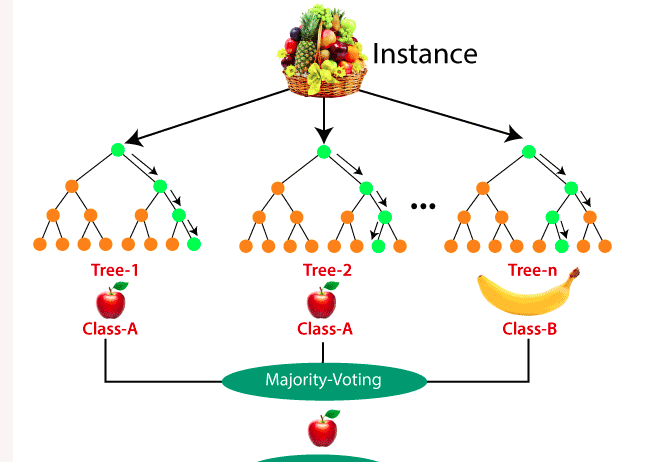
\includegraphics[width=14cm]{images/foret.png}
      \caption{Forêt aléatoire.\label{fig:foretaleatoire}}
    \end{center}
  \end{figure}


   \subsubsection{Echantillonage aléatoire des données d'entrainement}

    Lors de la phase d'entrainement, chaque arbre d'une forêt aléatoire apprend
    à partir d'un échantillon aléatoire de données. Les échantillons sont tirés 
    avec remplacement, connu sous le nom de \og bootstrapping \fg, ce qui 
    signifie que certains échantillons seront utilisés plusieurs fois dans un 
    seul arbre.

    Les prédictions sont faites en faisant la moyenne des prédictions de chaque
    arbre de décision. Cette procédure est connue sous le nom de \textit{bagging}
    abbréviation de \textit{bootstrap aggregating}

   \subsubsection{Fractionnement des noeuds}

    Le deuxième concept principal de la forêt aléatoire est que seulement un
    sous-ensemble de toutes les caractéristiques est pris en compte pour 
    diviser chaque noeud d'un arbre de décision. Cette valeur est 
    habituellement la raçine carré du nombre de caractéristiques pour une
    classification. Ainsi si nous avons 25 caractéristiques seulement 5
    seront pris aléatoirment pour diviser le noeud.

  \subsection{Les hyperparamètres dans les forêts aléatoires}

  Les hyperparamètres de la forêt aléatoires sont utilisés pour augmenter le
  pouvoir prédictif du modèle, soit pour rendre le modèle plus rapide.

  \subsubsection{Augmenter le pouvoir prédictif du modèle}

  Plusieurs hyperparamètres permettent d'augmenter le pouvoir de prédiction du
  modèle;
  \begin{description}
    \item[n\_estimators: ]Il s'agit du nombres d'arbres que l'algorithme
      construit avant de prendre le vote maximum ou la moyenne des prédictions.
      En général, un nombre d'arbres élevé augmente la performance et rend les
      prédictions plus stables mais ralentit également le calcul.
    \item[max\_features: ]Il s'agit du nombre maximum de caractéristiques qu'une
      forêt aléatoire considère pour diviser un noeud.
    \item[min\_sample\_leaf: ] Il s'agit du nombre minimum de feuilles nécessaires
      pour diviser un noeud interne.
  \end{description}

  \subsubsection{Augmenter la vitesse d'exécution du modèle}

  Les hyperparamètres permettant d'accélérer le modèle sont les suivants:
  \begin{description}
    \item[n\_jobs: ] Il indique au moteur le nombre de processeurs qu'il est autorisé
      à utiliser. Une valeur de $-1$ signifie qu'il n'y a aucune limite sur le
      nombre.
    \item[random\_state: ] Il rend la sortie du modèle reproductible. Le modèle
      produira toujours les mêmes résultats si on lui donne les mêmes
      hyperparamètres et les mêmes données d'entrainement.
    \item[oob\_score: ] Il s'agit d'une méthode de validation croisée des forêts
      aléatoires. Dans cette échantillonage, environ un tiers des données n'est
      pas utilisé pour entrainer le modèle mais plutôt pour évaluer ses
      performances sans aucune charge de calcul supplémentaire.
  \end{description}


\subsection{Les avantages et les inconvénients du modèle des forêts aléatoire}

\subsubsection{Avantages}
\begin{itemize}
  \item Les forêts aléatoires permettent de surmonter le problème de
    sur-ajustement en faisant la moyenne ou en combinant les résultats de
    diffrents arbres de décisions.
  \item Les forêts aléatoires fonctionnent mieux sur un large éventail de
    données qu'un seul arbre de décision.
  \item Les forêts aléatoires présentent moins de variance qu'un arbre de
    décision unique
  \item Les forêts aléatoires possèdent une très grande précision.
  \item Les algorithmes de forêt aléatoire maintiennent une bonne prédiction
    même si certaines informations sont absentes.
\end{itemize}

\subsubsection{Inconvénients}
\begin{itemize}
  \item La complexité est le principal inconvénient des algorithmes de Random
    Forest.
  \item La construction de forêts aléatoires est beaucoup plus
    difficile et longue que celle des arbres de décision.
  \item Il faut davantage de ressources de calcul pour mettre en oeuvre
    un algorithme de forêt aléatoire.
  \item Il est moins intuitif dans le cas où nous disposons d'une grande
    collection d'arbres de décision.
  \item Le processus de prédiction utilisant les forêts aléatoires est très long
    par rapport aux autres algorithmes.
\end{itemize}





\section*{Conclusion}

Ce chapitre nous a permis de présenter le machine learning et quelques algorithmes 
de classifications. En outre, nous nous sommes attardés sur les arbres de décisions 
qui sont un type de classifieurs qui nous pensons sont adaptés au contexte de notre étude.
Maintenant, nous poursuivrons en  présentent la conformité dans le domaine bancaire.
 
\glsresetall
\chapter{La conformité dans le secteur bancaire}
\section*{Introduction}
Dans ce chapitre, nous élaborerons d’abord une étude de l'existant. Pour celà, 
nous présenterons quelques plateformes permettant d'analyser 
des opérations de transferts de fonds. Après cela, Nous étudierons la fonction conformité ou 
compliance en anglais dans le secteur bancaire. 


\section{Etude de l'existant}
\subsection{Analyse des dossiers de transfert à la SGBF}

Le problème posé au niveau du service OPI, c'est l'analyse en temps réel des
dossiers de transferts reçus au niveau du guichet. Cette analyse suit un
processus.
La première phase de ce processus est la réception du dossier.
A la réception du dossier, le collaborateur analyse la cohérence du dossier.
Cette analyse consiste en la vérification de la cohérence et l'exactitude des
informations contenues sur les éléments constitutifs du dossier.

Après cette phase, le collaborateur analyse la complétude du dossier. Une fiche,
disponible au niveau du guichet permet aux collaborateurs de OPI de savoir à vue
d'oeil quels justificatifs devraient être présent dans le dossier en fonction du
motif de l'opération.

L'étape suivante est la vérification de la fiabilité des différents acteurs de l'opération
à travers des outils comme Force-online.

La dernière étape concerne la vérification du circuit de transfert. Il s'agit à cette étape
de s'assurer que la règlementtion autorise l'opération qui est entrain d'être menée entre les diffrents acteurs.

\subsection{Plateformes existantes dans le milieu bancaire}

De nombreuse plateformes permettent de juger le risque de non-conformité d'un acteur d'une
opération de transfert. Ces plateformes sont toutes propriétaire.

\subsubsection{ComplianceBond}

\textbf{ComplianeBond} est un des produits de la plateforme HighBond. HighBond
est une plateforme logicielle de gouvernance d'entreprise qui renforce la 
sécurité, la gestion des risques, la conformité et l'assurance. ComplianceBond
est une solution de gestion de la conformité qui permet aux organisations de
mettre en oeuvre, d'automatiser et de démontrer une assurance par rapport à un
programme de conformité.

Les fonctionnalités principales de ComplianceBond sont les suivantes:
\begin{itemize}
  \item Centraliser la documentation des besoins et des contrôles mappés. Cela
    permet de réduire le temps passé à documenter et à tester la conformité.
  \item Evaluer et surveiller la conformité en automatisant les tests de
    surveillance de conformité en temps réel.
  \item Rapport sur le statut de conformité
\end{itemize}
Il s'agit d'une plateforme propriétaire.

\subsubsection{TraProtect} 

TraProtect de TraInvestment est une plate-forme multicanal, multi-activité et
multi-niveau de prévention temps réel et détection de la fraude des 
transactions spécialement conçue pour le monitoring des transactions de 
paiement électronique. Elle est destinée à toute institution traitant les 
transactions de paiement électronique.

\subsubsection{ kdprevent}

La plateforme kdprevent permet de lutter contre le blanchiment d'argent et le 
financement du terrorisme. Elle a été mise en œuvre dans plusieurs pays du 
monde, dans plus de 50 institutions. Elle  est conçue pour détecter les 
activités inhabituelles, inattendues et suspectes. Une fois détectée, elle 
envoie automatiquement des avertissements aux responsables, généralement les 
responsables conformité.
Ses principales fonctionalités sont:
\begin{itemize}
  \item Analyse d'une transaction unique et d'un ensemble de transactions 
    liées qui ont eu lieu dans une période de temps donnée.
  \item Détection automatique et interruption des transactions suspectes
    (i.e SWIFT, SEPA, SIC, etc.) et notification en temps réel.
  \item Génération d'alertes pour les situations suspectes détectées
  \item Un analyseur de relations qui vous permet d'explorer les relations 
    potentiellement suspectes ou inconnues qui existent entre les clients,
    les emprunteurs ou les comptes.
\end{itemize}


\section{La conformité ou compliance}

Le cadre règlementaire autour des activités financières a été fortement
renforcé, faisant de la conformité (ou Compliance) un pilier indispensable
de la protection des institutions financières en particulier les banques 
et de leurs clients. \cite{arnaud2015}

  \begin{figure}[h!]
    \begin{center}
      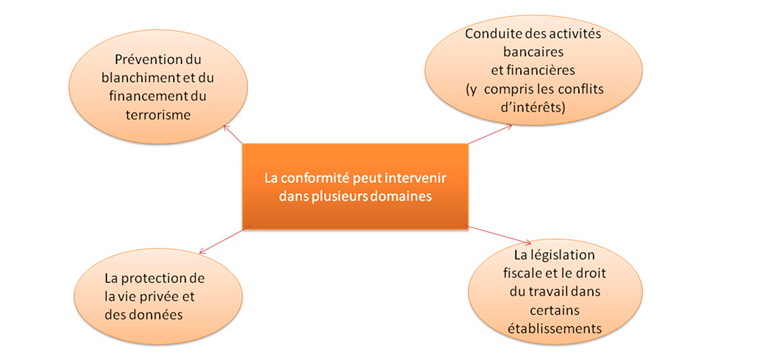
\includegraphics[width=14cm]{images/domaineconformite.png}
        \caption{Domaine d'intervention de la conformité
        .\label{fig:domaineconformite}}
    \end{center}
  \end{figure}

\subsection{Définition}
La conformité en anglais compliance est un concept qui a fait naître de 
nouvelles obligations pour le banquier. En effet, face à la complexité des
environnements et à \og l'inflation règlementaire\fg,  la fonction 
conformité a pour but de prévenir tout risque de non-conformité des opérations
bancaires et financières. La conformité se définit donc comme l’obligation 
de veiller à ce que les collaborateurs des différentes banques s’assurent en
permanence que soient respectées:
\begin{itemize}
  \item Les dispositions législatives et règlementaires propres aux activités
    bancaires;
  \item Les normes et usages professionnels et déontologiques ;
   \item Les codes de conduites notamment le code éthique et les procédures internes
\end{itemize}

Dans ses grandes lignes, la conformité consiste à:
\begin{itemize}
  \item Identifier et à jauger le degré de non-conformité d’une entité 
    économique par rapport à l’ensemble des règles de conduite qui lui sont
    applicables
  \item Mesurer son taux d’exposition aux risques de sanction judiciaire et
    administrative
  \item Evaluer les pertes financières qu’elle pourrait subir
  \item Conseiller une entité économique pour qu’elle se mette en 
    conformité avec les normes législatives et règlementaires.
\end{itemize}

En somme, la conformité est l’ensemble des actions visant
à l’intégration, dans la structure bancaire des exigences issues des 
règlementations financières.  La fonction conformité dans une banque
recouvre quatre grandes activités :

\subsubsection{Sécurité financière}
Elle est attentive à la sécurité financière de la banque et lutte en ce sens 
contre la fraude, le blanchiment de capitaux et financement du terrorisme, 
les abus de marché et les embargos.

\subsubsection{La protection Clientèle}
Elle assure en parallèle, une protection continue de la clientèle en
préservant aussi bien leurs intérêts propres, que ceux des marchés ou de la 
banque elle-même.

\subsubsection{Le contrôle permanent}

Elle appartient au dispositif global de contrôle permanent et assure la
gestion des risques de non-conformité.

\subsubsection{La déontologie}

La déontologie est également une partie intégrante de la conformité. Elle
permet de s’assurer du respect du recueil des règles de déontologie de 
l’établissement bancaire ainsi que de traiter les signalements pouvant 
provenir de tous les collaborateurs de la banque.

\subsection{Rôle de la conformité dans le domaine bancaire}

Le rôle de la conformité est d’abord de donner aux dirigeants de la Banque 
ainsi qu’au Conseil d'administration l'assurance raisonnable que les risques 
de non-conformité réglementaires et de réputation sont dûment surveillés, 
contrôlés et atténués au niveau du Groupe. C’est également s'assurer en 
permanence que les lois et réglementations ainsi que les règles et normes 
internes définies par les pays sont respectées. In fine, il s’agit d’offrir 
aux clients l’assurance d’un environnement sécurisé pour réaliser leurs 
opérations financières, en vérifiant que celles-ci sont conformes aux règles 
déontologiques et aux législations.

\section{Présentation du cadre règlementaire}

La SGBF est membre d'un groupe international français. Elle est donc soumise
aussi bien aux règlements de la zone UEMOA qu'à celles européennes et 
internationales.

Au niveau international, l'organisme de référence de contrôle est le GAFI.
Le GAFI (Groupement d'Action FInancière) est un organisme international, sous
l'égide des nations unies, créé à Paris en  1989. Il a pour rôle d'émettre des
recommandations dans le domaine de la lutte contre le blanchiment des capitaux
et dans la lutte contre le financement du terrorisme. Les pays membres du GAFI
acceptent de fait les recommandations et s'engagent à mettre en oeuvre les lois
permettant l'application de ces recommandations. Les pays membres du GAFI
s'engagent également à s'auto-évaluer à intervalles de temps réguliers dans le
but d'améliorer leurs dispositifs respectifs.
Il s'agit aujourd'hui la référence principale dans le domaine de l'AML (Anti
Money Laundering).

Les contrôles de la fonction conformité regroupent aussi bien ceux sur la
règlementation de change que ceux sur les composantes d'un programme AML
\nomenclature{AML}{Anti Money Laundering}.

\subsection{ La règlementation de change} 

La règlementation de change est un outil juridique important non seulement
dans le monde des affaires, mais aussi dans la vie d’un pays compte tenu de
la diversité des phénomènes économiques et de la criminalité qui pourrait
se développer dans ce domaine. Elle relève de la tutelle du Ministre chargé
des Finances. Elle prescrit que les règlements financiers et mouvements de 
capitaux entre l'UEMOA et l'Etranger, ainsi que les opérations de change manuel
dans l'UEMOA, ne peuvent s'effectuer que par l'entremise de la BCEAO ou d'une 
banque intermédiaire agréé\cite{reglementfin}.

Le Change se définit comme l’échange d’une monnaie contre une autre, C’est le 
bénéfice réalisé sur la différence des cours entre deux monnaies. C’est aussi 
le taux de conversion entre deux monnaies.

Au Burkina Faso et dans les pays membres de l’UEMOA, les transferts à 
l’étranger sont régis par un ensemble de texte. Ces textes fixent les 
procédures à suivre par les intermédiaires agréés en matière d’exécution des
opérations avec l’étranger et déterminent la procédure de domiciliation et de 
règlement des importations par la banque.

\subsubsection{La règlementation de change sur les opérations d'exportation}

Les opérations d'exportations d'un montant supérieur à 500000 sont soumises à
domiciliation auprès d'une banque. Pour chaque opération 
d'exportation, les résidents sont tenus d'encaisser les recettes en devises 
et de les céder à la banque domiciliataire dans un délai d'un mois à compter
de la date d'exigibilité du paiement.
 
\subsubsection{La règlementations de change sur les opérations d'importation}

Les opérations d'importation de marchandises étrangères, c'est-à-dire originaires
d'un pays extérieur à la zone franc, doivent être domiciliées auprès d'une banque
intermédiaire agréé, lorsque leur valeur dépasse un certain seuil variable selon 
les pays.\cite{reglementfin}
Pour une opération d'importation, le dossier complet de domiciliation doit contenir
une copie de la facture établi par le fournisseur, une attestation d'importation,
et un formulaire d'autorisation de change.
 
\subsubsection{La règlementation de change sur les opérations d'investissement et
d'emprunt}
La règlementation de change exige que pour tout investissement, prêt, ou
opération en capital par un résident, une autorisation préalable du ministère
chargé des finances est obligatoire.
 
\subsection{Les composantes d'un programme AML}

Les programmes AML permettent de garantir la sécurité financière d'un
établissement financier. Ce sont:
 \begin{enumerate}
   \item Lutte contre le blanchiment des capitaux
     (AML/LAB)\nomenclature{LAB}{Lutte Anti Blanchiment}
   \item Lutte contre le financement du terrorisme
     (CFT)\nomenclature{CFT}{Contre le Financement du Terrorisme}
   \item Respect des embargos commerciaux et financiers
   \item Surveillance des opérations de marché
 \end{enumerate}
 
 \subsubsection{La lutte contre le blanchiment de capitaux} 

\textbf{Le blanchiment de capitaux} consiste à dissimuler la provenance d'argent acquis
de manière illégale, appelé communément \og{}argent sale\fg{}, en lui donnant
l'apparence de fonds d'origine licite(\og{}argent propre\fg{}) pour le
réinvestir dans des activités légales.
Le Blanchiment permet notamment aux criminels de masquer une augmentation
trop ostensible de leur richesse afin d'éviter d'attirer l'attention des autorités.
On distingue trois phase dans le processus global de blanchiment:
\begin{description}
  \item[\textbf{La phase de placement}] qui consiste à injecter dans le système financier
    les sommes d'argent issues des crimes et des délits; 
  \item[\textbf{La phase d'empilement}] qui consiste à brouiller les pistes. Le but est 
    d'effectuer un ensemble de transactions qui ont pour objectif d'empêcher 
    toute traçabilité des mouvements de fonds pour remonter à l'opération 
    d'origine.
  \item[\textbf{La phase d'intégration}] qui consiste à réinvestir les fonds
    dans des placements honorables: biens immobiliers, titres, participations
    financires dans les entreprises.
\end{description}

Lutter contre le blanchiment de capitaux reviendrait donc à mettre 
en place des mesures d vigilance au niveau des acteurs sociaux et économiques
pour que les étapes à franchir pour blanchir les capitaux soient difficiles
voire impossible. \cite{reglementaml}

\subsubsection{La lutte contre le financement du terrorisme}

\textbf{Le financement du terrorisme} consiste à fournir ou réunir des fonds,
des biens ou des services susceptibles d'être utilisés dans le but de facilité
ou de perpétrer des actes de terrorisme.
Ces opérations à finalité criminelle impliquent parfois des fonds d'origine
parfaitement légale.
Alors que le blanchiment des capitaux est une opération financière qui vise 
à cacher l'origine des fonds, le  financement du terrorisme, au contraire,
utilise des techniques pour tenter de cacher la destination des fonds.

La lutte contre le financement du terrorisme s'effectue par identification et
contrôle du donneur d'ordre, du destinataire effectif de la transaction, et 
ceci par filtrage par rapport à des listes de sanctions officielles.

\subsubsection{Le respect des embargos commerciaux et financiers}

La communauté internationale, au travers de l'Organisation des Nations Unies 
(ONU), s'est dotée d'un arsenal juridique pour permettre le contrôle des flux
monétaires. Parmi certaines mesures figure l'embargo commercial. \textbf{Un embargo} 
(généralement partiel), vise à restreindre les relations des pays membres
avec le pays concerné et à encadrer strictement ce qu'il est permis de faire
ou non en matière de commerce et d'échange. Les embargos se traduisent 
généralement par des mesures d'interdiction de certains types d'opérations, 
comme par exemple l'interdiction de commercer sur du matériel d'origine 
nucléaire ou militaire, ou encore l'interdiction d'exporter les ressources 
pétrolières d'un pays sous embargo.

\subsubsection{La surveillance des opérations de marché}

Il s'agit d'une obligation qui vise à s'assurer que la banque ou l'établissement
financier n'utilise pas son accès privilégié aux marchés financier pour en tirer
profit au détriment de ses clients. La surveillance des marchés regroupe les
fonctions suivantes:
\begin{description}
  \item[Les délits d'initiés:]
    Pratique consistant à profiter indument d'une information privilégiée avant
    que celle-ci ne soit rendue publique. Une information privilégiée est une 
    information précise sur un émetteur qui, si elle était rendu publique, 
    serait susceptible d'influencer le cours de certains instruments 
    financiers.
  \item[Les manipulation de marché: ]
    Cette problématique vise à s'assurer que la banque ou l'établissement 
    financier n'utilise pas son poids financier et son effet de levier sur 
    certains titres pour faire évoluer le marché dans un sens qui lui est 
    favorable. 
  \item[La résolution des conflits d'intérêts: ]
    Cette dernière problématique vise à identifier les éventuels conflits 
    résultant de la multiplicité des activités bancaires au sein d'un grand
    groupe financier.
\end{description}

\section{Machine Learning et mise en oeuvre d'un programme de conformité}

Après avoir présenté les composantes d'un programme AML, nous allons analyser
les moyens à mettre en oeuvre au sein des établissements de crédit pour 
appliquer de manière opérationnelle les recommandations du GAFI
\nomenclature{GAFI}{Groupe d'Action FInancière} et surtout 
comment ces moyens pourraient être automatisés grâce au ML.
 
\subsection{Le Machine Learning pour la simplification des procédures KYC}
 
KYC \nomenclature{KYC}{Know Your Customer} est l'acronyme de Know Your Customer. Il désigne le processus permettant 
de vérifier l'identité des intervenants à une opération bancaire afin de 
s'assurer de la conformité des clients face aux législations anti-corruption,
de leur probité et de leur intégrité.

Initialement mise en oeuvre par une intervention humaine, les tâches 
répétitives des procédures KYC pourraient être automatisées grâce au 
Machine learning. Les principales étapes de la procédure KYC qui peuvent être
automaisées par des modèles d'apprentissage automatiques sont:
  
  \subsubsection{L'identification et le contrôle des informations 
    d'identification des clients}
    Il s'agit au cours de cette étape de demander et d'enregistrer les
    informations personnels du clients et de contrôler son identité par rapport
    à une pièce d'identité officielle. A ce niveau, les informations
    personnelles nom, prénoms, date de naissance, situation maritale,
    adresse\ldots dites \og bio data \fg sont demandées.

    Le contrôle des informations d'adresse nécessitera la fourniture par le 
    client d'une pièce probante (facture d'eau, de téléphonie fixe, etc.).
    La banque pourra également adresser un courrier de bienvenue ou de 
    remerciement pour la fidélité au client  et vérifier que le courrier ne
    revient pas.

  \subsubsection{Le contrôle des clients par rapport aux listes de sanctions}
    Lors de toute opération, la banque contrôle la présence éventuelle d'un
     des intervenants de l'opération sur une ou plusieurs listes de 
    sanction, selon la réglementation en vigueur dans le pays. Ces listes sont
    établies par les autorités officielles(nationales ou supranationales comme
    L'ONU, L'Union Européenne). Elles regroupent des individus ou de groupes qui
    compte tenu de leur activités ont été frappé de mesure d'embargo nominative.

  \subsubsection{Qualification du risque de blanchiment}
    Il s'agit là de vérifier si le client n'existe pas sur des listes qui ne 
    sont pas d'ordre public. Ces listes peuvent être celles des PEP
    \nomenclature{PEP}{Personnes Exposées Politiquement} ou une liste d'indésirables car en opposition 
    avec la déontologie et les valeurs du groupe financier.

  \subsubsection{Consignation des pièces d'identification des clients}
    Après la phase d'identification du client et de son contrôle, 
    l'établissement financier doit enregistrer les preuves d'identification du
    client et les archiver.

    
\subsection{Le Machine Learning, un outil essentiel à la détection des 
 transactions suspectes}
 
 La lutte contre le blanchiment d'argent et le financement du terrorisme est
 principalement basée sur l'élaboration, par des algorithmes, de scénarios
 d'anticipation dits « déterministes ». Les algorithmes utilisés analysent
 en temps réel les transactions et sont capables, en quelques instants, de
 décéler une transaction suspecte. Ces scénarios se basent sur des règles
 arrêtées, constantes et ne sont que très peu modifiés une fois mis en 
 place. La procédure est basé sur des mots clés et il est difficile de calibrer
 ces logiciels à un niveau permettant une protection optimale face aux 
 transactions frauduleuses sans générer pour autant un nombre élevé de fausses
 alertes qui de ce fait viendrait perturber les activités de conformité.

 Pour résoudre ces problémes particulièrement chronophages et coûteux pour les
 banques, des applications basées sur le Machine Learning pourraient apprendre
 à identifier les transactions frauduleuses en établissant des procédés 
 standardisés et automatisés. Cela permettra de réduire la charge de travail des
 équipes, tout en affinant la précision de l'analyse. Il s'agirait là pour les
 banques de réduire leurs coùts et leur sanctions, tout en assignant un travail
 à plus forte valeur ajoutée aux équipes chargées de la conformité.


\section*{Conclusion}
Le blanchiment d'argent, la lutte contre le terrorisme sont des fléaux dangereux
et il est du devoir des banques de lutter efficacement contre ces pratiques. Aux
collaborateurs de la SGBF, il est demandé de:
\begin{itemize}
  \item Appliquer impérativement la règlementation française(exigence du groupe)
  \item se conformer à la règlementation du Burkina Faso applicable à leur
    égard. Si Celle-ci est plus restrictive, elle s'applique en priorité tout en
    restant conforme avec les autres exigences du groupe.
  \item Appliquer la règlementation américaine pour toute
    transaction vers les Etats-Unis ou impliquant le dollar Américain.
\end{itemize}

Ce chapitre nous a permis de présenter la conformité dans le domaine bancaire,
et les facilités qu'apporterait l'apprentissage automatique dans sa mise en 
oeuvre dans un établissement financier. La suite sera
consacrée à l'implémentation et à la présentation des résultats.

 
\glsresetall
\chapter{Approche et Implémentation}

\section*{Introduction}
Dans ce chapitre nous présenterons premièrement les données qui ont été utilisés
pour entrainer notre modèle. Ensuite, nous présenterons les résultats obtenus à
la suite de l'utilisation des algorithmes sur nos données. Enfin nous 
présenterons les perspectives envisagées.
Quelle approche est la mieux adaptée à nos besoins? Choisir un algorithme 
d’apprentissage supervisé ou non supervisé dépend habituellement de 
facteurs liés à la structure et au volume de nos données, et le cas 
d’utilisation auquel nous voulons l’appliquer.


\section{Approche}

L'objectif de notre travail est de mettre en place un système permettant 
d'analyser ou de réaliser la mise en conformité d'une opération à l'étranger et
de tous les acteurs intervenants dans cette opération. Cette analyse se base
sur le dossier que le client a fourni au guichet des opérations 
internationales.

L'analyse conformité regroupe plusieurs activités que nous ne considèrerons pas
toutes dans un premier temps. En effet, dans le but d'avoir un modèle
beaucoup plus efficace, nous nous focaliserons tout d'abord sur :
\begin{itemize}
  \item La détection des transactions suspectes
  \item l'allègement des procédures KYC
\end{itemize}
Pour atteindre les objectifs que nous nous sommes fixés, nous considérons un
dossier d'opération comme l'ensemble des informations contenues sur chaque
élément du dossier. Un dossier d'opération est donc l'ensemble des
caractéristiques entrant en compte dans la détection d'une transaction suspecte
et des informations d'identification de tous les intervenants à l'opération.
Ces informations sont relevées directement sur le dossier physique transmis 
par le client.

La détection d'anomalies dans notre cas n'a pas fourni de résultats 
satisfaisants. En effet, elles éliminent une énorme partie des données d'entrées, qui
ne représentent pas forcément des anomalies. Nous avons donc chercher d'autres
méthodes pour la résolution de notre problème.
Pour cela, la méthode adoptée pour la mise en place du système devra respecter les
exigences bancaires à savoir que la mise à jour du sytème doit être 
possible et la décision prise expliquable et le système sécurisé.
En somme, le modèle ne devra pas fonctionner comme une boîte noire.

Parmi les principaux algorithmes de classification connus, ceux ne
fonctionnant pas comme une boite noire sont l'algorithme des plus proches
voisins(K-NN) et celui des arbres de décisions(Décision Tree). Les arbres de
décisions offrent l'avantage de pouvoir générer des règles de décisions pour
toutes les différentes classifications qui sont réalisées. C'est la méthode qui
sera utilisée pour réaliser notre modèle d'apprentissage.

Nous posons comme hypothèse de départ que tous les dossiers sont complets et 
conformes à la règlementation de change avant de passer par le modèle
d'aprentissage. Cette hypothèse nous permet de nous focaliser sur les autres
aspects de la conformité qui ont été cités précédemment.

\section{Réalisation}

\subsection{Le jeu de données}

\subsubsection{Acquisition des données}

Les moyens à mettre en oeuvre au sein des banques pour appliquer de manière
opérationnelle les recommandations du GAFI et se conformer ainsi aux
réglementations en vigueur (ordonnance 2009-104, code monétaire et financier)
implique un processus approfondi de connaissance du client et le contrôle et
la surveillance des transactions.

Les éléments présents sur un dossier et permettant de connaitre un client
intervenant dans une opération(client émetteur ou destinataire de l'opération)
sont:
\begin{itemize}
  \item le type de personne (personne physique ou morale)
  \item l'identité de la personne
  \item le pays de résidence de la personne
  \item la banque de la personne
  \item le pays dans lequel cette banque se trouve
\end{itemize}
Tous les éléments cités ci-dessus doivent être contrôlés sur les listes
officielles de vérification de sanctions et d'embargo. Le résultat de chacun
de ces contrôles est indispensable pour effectuer l'analyse d'une opération.

Les informations présentes sur un dossier et permettant de contrôler ou
surveiller une transaction en cours sont:
\begin{itemize}
  \item L'activité de l'émetteur de l'opération
  \item l'activité du bénéficiaire de l'opération
  \item l'objet de l'opération(salaire, achat d'une voiture, de frais
    médicaux\ldots)
  \item le type de l'opération(transfert émis, transfert recu,  credoc,
    remdoc\ldots)
  \item le montant de l'opération
  \item la dévise de l'opération
\end{itemize}

En somme, Pour inférer correctement sur de nouvelles données, les jeu de
données qui seront utilisés pendant la phase d'apprentissage auront les
caractéristiques suivantes :

\begin{itemize}
  \item le type de personne du donneur (personne physique ou morale)
 \item l'identité de l'émetteur et le résultat de son contrôle sur les
   listes de sanctions
 \item le pays de résidence de l'émetteur et sa notation
 \item la banque de l'émetteur et le résultat de son contrôle sur les
   listes de sanctions
 \item le pays dans lequel cette banque se trouve et sa notation
 \item le type de personne du bénéficiaire (personne physique ou morale)
 \item l'identité du bénéficiaire et le résultat de son contrôle sur les
   listes de sanctions
 \item le pays de résidence du bénéficiare et sa notation
 \item la banque du bénéficiaire et le résultat de son contrôle sur les
   listes de sanctions
 \item le pays dans lequel cette banque se trouve et sa notation
 \item l'activité de l'émetteur de l'opération
 \item l'activité du bénéficiaire de l'opération
 \item l'objet de l'opération(salaire, achat d'une voiture, de frais
    médicaux \ldots
 \item le type de l'opération(transfert émis, transfert recu,  credoc,
    remdoc...)
 \item le montant de l'opération
 \item la dévise de l'opération
\end{itemize}

Comme nous ne disposions pas de toutes ces informations sur des fichiers, nous
avons, en collaboration avec les colaborateurs du service des opérations
internationales et ceux de la Direction Conformité, constitué un jeu de données
afin de réaliser notre apprentissage.


\subsection{Prétraitrement des données}

Les caractéristiques recencées ci-dessus nous permettent de juger de la 
conformité d'un dossier de transferts. Certaines caractéristiques sont très
distinctives et pourraient entrainées un sur-apprentissage de notre modèle.
Il s'agit par exemple de 
\begin{itemize}
  \item l'identité de l'émetteur de l'opération
  \item le pays de résidence de l'émetteur 
  \item la banque de la l'émetteur
  \item le pays dans lequel cette banque se trouve
  \item l'identité du bénéficiaire de l'opération
  \item le pays de résidence du bénéficiaire de l'ordre
  \item la banque du bénéficiaire
  \item le pays dans lequel cette banque se trouve
  \item la dévise de l'opération
\end{itemize}

Dans le tableau \ref{tab:tab3}, nous présentons l'ensemble des caractéristiques de
notre jeu de données. Celles qui sont en italiques représentent les 
caractéristiques d'entrée de notre algorithmes de machine learning.


\begin{table}

  \begin{center}
    \begin{scriptsize}
      \renewcommand{\arraystretch}{2}
      \begin{tabular}{|c|l|l|}
        \hline
        \rowcolor[gray]{.7}
        \bf \rule[-0.4cm]{0mm}{1cm} Section & \bf Caractéristiques & \bf Exemples\\
        \hline
        \multirow{7}{*}{\bf Emetteur de l'ordre} & \textit{Type de personne} & Personne 
        physique 
        \tabularnewline
        & Identité & XXXXXX XXXXXX \tabularnewline 
        & \textit{Résultat du contrôle de l'émetteur} & Aucune sanction  \tabularnewline
        & Pays de résidence & Burkina Faso \tabularnewline
        & \textit{Notation du pays de résidence} & LOW \tabularnewline
        & Banque de l’émetteur & SGBF \tabularnewline
        & Pays de la banque & Burkina Faso \tabularnewline
        & \textit{Notation Pays de la banque} & LOW \tabularnewline
        & \textit{Résultat du contrôle sur la banque} & Aucune sanction  \tabularnewline
        & \textit{Activité de l'emetteur} & Activités extractives \tabularnewline 
        \hline

        \multirow{7}{*}{\bf Bénéficiaire de l'ordre} & \textit{Type de personne} & Personne
        morale 
        \tabularnewline
        & Identité & ZZZZZZZZZZ \tabularnewline
        & \textit{Résultat du contrôle sur la personne} & Aucune sanction  \tabularnewline
        & Pays de résidence & France \tabularnewline 
        & \textit{Notation du pays de résidence} & LOW \tabularnewline
        & Banque de l’émetteur & BNP Paribas \tabularnewline
        & Pays de la banque & France \tabularnewline 
        & \textit{Notation Pays de la banque} & LOW \tabularnewline
        & \textit{Résultat du contrôle de la banque} & Aucune sanction  \tabularnewline
        & \textit{Activité du bénéficiaire} & Hébergement et hôtellerie  \tabularnewline 
        \hline
        \multirow{5}{*}{\bf Opération} & Type  & Règlement de facture \tabularnewline
        & \textit{Objet}  & Frais d'hébergement \tabularnewline
        & \textit{Montant}& 25000 \tabularnewline
        & Devise & Euros \tabularnewline

        \hline
      \end{tabular}
    \end{scriptsize}
    \caption{Exemple de dossier d'opération conforme \label{tab:tab3}}
  \end{center}
\end{table}


Le jeu de données final qui a servi pour l'apprentissage et les tests  est constitué de
six cent (600) dossiers d'opérations.


Pour des questions pratiques, nous avons constitué un dictionnaire des
différents secteurs d'activités ainsi que des objets de transactions.
Un échantillon du dictionnaire est présenté au tableau \ref{tab:codage}.
\begin{table}
 \begin{center}
    \begin{scriptsize}
      \renewcommand{\arraystretch}{2}
      \begin{tabular}{|m{5cm}|m{2cm}||m{5cm}|m{2cm}|}
        \hline
        \rowcolor[gray]{.7}
        \bf \rule[-0.4cm]{0mm}{1cm} Libellé secteur d'activité & \bf Code &
        \bf Libelle du secteur d'activité & \bf Code \\
        \hline

      Activités extractives & 0 &  Activités financières & 15 \\
      Agriculture et chasse & 1 & Hôtels et restauration & 3 \\
      Industrie & 4 & Activites de ménages & 5 \\
      Activités des organisations extraterritoriales & 6 & Activités financières & 7 \\
      Commerce gros & 8 & Santé et action sociale & 8 \\
      Administration publique & 9 & Commerce détail\\
      Transport & 10 & Education & 11 \\
      Développements logiciels & 12 & Maintenance de materiels informatiques & 13\\
      Fabrication Produits pharmaceutiques & 16 & Construction & 17 \\
      Fabrication de meubles & 18 & Activités associatives & 19 \\
      Commerce détail & 20 & Fabrication chaussures & 21 \\
      Télécommunications & 22 & Activités Juridiques & 23 \\
      Fabrications produits alimentaires & 24 & Service immobilier & 25 \\
      Fabrication de boissons & 26 & Pêche et pisciculture & 27 \\
        \hline
      \end{tabular}
      \end{scriptsize}
      \caption{Codage de quelques secteurs d'activités\label{tab:codage}}
  \end{center}
\end{table}

    \subsection{Validation croisée et stratification des données}

    \subsubsection{Validation croisée}
      Pour nous assurer que notre modèle ne souffre pas de sur-apprentissage, et
      qu’il saura faire des prédictions sur de nouvelles données, nous avons
      implémenté la validation croisée sur notre modèle de Decisions Tree. La 
      validation croisée va nous permettre d’utiliser l'intégralité de notre jeu
      de données pour l’entraînement et pour la validation.

      Pratiquement, il s'agit de dcouper le jeu de données en $k$ parties(folds
      en anglais) à peu près égales. Tour à tour, chacune des $k$ parties est
      utilisée comme jeu de test. Le reste(autrement dit l'union de $k-1$ autres
      parties) est utilisé pour l'entrainement.
      La validation croisée permet d'éviter un biais potentiel lié au fait de
      faire une évaluation unique.

      \subsubsection{Stratification}


    Le jeu de données dont nous disposons n'est pas équilibré i-e le nombre de
    dossiers non conformes est plus élevé que celui des dossiers conformes. La
    stratification permet d'éviter que les données d'entrainements ne
    contiennent que des exemples positifs et les données de test que des
    exemples négatifs, ce qui affecte négativement les performances du modèle.


\subsection{Les outils}
Nous allons présenter quelques outils qui nous ont permis de mettre en place
le modèle et la plateforme que nous avons proposée. Chaque étape dans la
mise en place d'un modèle de machinelearning possède des outils spécifiques
associés.
\subsubsection{Le langage python}
\begin{wrapfigure}[5]{l}{3.5cm}
  \vspace{-7mm}
  
\includegraphics[width=3cm]{images/python.png}
\end{wrapfigure}

Python a été utilisé pour les codes d'implémentation de notre
modèles. Il s'agit d'un langage de programmation, dont la première version 
est sortie en 1991. Ce langage a été baptisé ainsi en hommage à la troupe de
comiques les \og Monty Python \og.
Python est un langage puissant riche en possibilités et dont les fonctionnalités
peuvent être étendues grâce à de nombreuses bibliothèques. Ainsi, nous avons
utilisé de nombreuses bibliothques python afin de mettre en oeuvre notre modèle.

\begin{description}
  \item[\textbf{Pandas et numpy: }] Pour le nettoyage et l'exploration de nos
      données, les librairies \textbf{Pandas} et \textbf{Numpy} ont été utilisées.
      Pandas permet de créer des tableaux ou dataframes à partir des données
      brutes.
    \item[\textbf{Scikit-learn: }] Tensorflow et Scikit-learn sont les librairies
        les plus utilisées pour la modélisation. Pour notre modèle, le choix a
        été fait d'utiliser \textbf{Scitit-learn}. Ce choix se justifie par le
        fait qu'il implémentedirectement et de manière didactique les différents
        algorithmes d'apprentissage automatique.
    \end{description}
\subsubsection{Le langage Javascript} 

\begin{wrapfigure}[5]{r}{3.5cm}
  \vspace{-7mm}
  
\includegraphics[width=3cm]{images/javascript.png}
\end{wrapfigure}
JavaScript est un langage de programmation de scripts principalement employé
dans les pages web interactives mais aussi pour les serveurs avec 
l'utilisation (par exemple) de Node.js. A travers le framework angular qui est
un framework Javascript, il nous a permis de réaliser une interface
conviviale qui permettrait l'utilisation de notre modèle.

\subsubsection{Flask}
\begin{wrapfigure}[5]{l}{3.5cm}
  \vspace{-7mm}
  
\includegraphics[width=3cm]{images/flask.png}
\end{wrapfigure}

Flask est un framework open-source de développement web en Python. Son but 
principal est d'être léger, afin de garder la souplesse de la programmation
Python, associé à un système de templates. Ils nous a permis de mettre à 
disposition de notre client javascript le modèle python qui a été implémenté.

\subsubsection{Jupyter Notebook}
\begin{wrapfigure}[5]{r}{3.5cm}
  \vspace{-7mm}
  
\includegraphics[width=3cm]{images/jupyter.png}
\end{wrapfigure}

Le Jupyter Notebook est une application web open-source qui vous permet de 
créer et de partager des documents contenant du code interprété en direct, 
des équations, des visualisations et du texte narratif. Les utilisations 
comprennent : le nettoyage et la transformation de données, la simulation 
numérique, la modélisation statistique, la visualisation de données, 
l'apprentissage machine, et bien plus encore. Il est l'un des outils  
du projet Jupyter.

\subsubsection{Visual studio code}

Visual studio code est un éditeur de code édité par microsoft. Il est utilisé
par les développeurs pour la progammer dans de nombreux langages de
programmation. 


 \section{Résultats}
Rappelons que l'objectif de notre étude est mettre en place un système
permettant de classifier une opération(dossier de transfert) à l'étranger selon
la conformité. Un tel système se compose de deux parties. La première partie est
un modèle de machine learning réalisé grâce aux algorithmes de décision Tree. La
seconde est une application permettant d'envoyer à partir d'un formulaire les
éléments du dossier au modèles de Machine Learning.

Nous présenterons tout d'abord les résultats du modèle. Par la suite, nous
montrerons l'application qui permettra une utilisation du modèle.

  \subsection{Résultats du modèle}
  Le modèle classe les dossiers opérations en deux groupes: un groupe
  représentant l'étiquette dossier conforme, l'autre représentant l'étiquette
  dossier non-conforme. Nous étiquettons un dossier conforme \textit{1} et un
  dossier non-conforme \textit{0}
  Les mesures détaillés des test par catégorie sont représentés sur les figures suivantes.

     \begin{figure}[h!]
        \begin{center}
          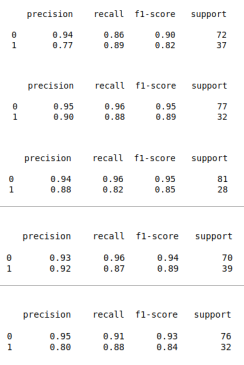
\includegraphics{images/all222.png}
          \caption{Résultat du test. \label{fig:result}}
        \end{center}
      \end{figure}

  Notre test nous révèle un f1-score toujours élevé pour les dossier étiquetés 0
c'est-à-dire pour les dossiers non-conformes. La moyenne de prédiction juste
globale est de $61.31\%$.

Les arbres de décisions étant considérés comme des classifieurs faibles, nous
avons appliqué sur nos données un modèle de forêts aléatoire afin de comparer
ces résultats avec ceux issus d'un arbre de décision simple.

Les résultats obtenues pour un modèle de forêt aléatoire sont présentés dans la 
figure ci-dessous. \ref{fig:randomresult}
 \begin{figure}[h!]
  \begin{center}
    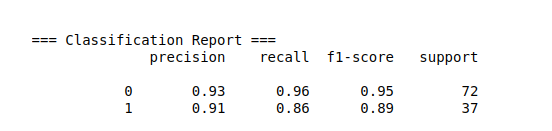
\includegraphics[width=14cm]{images/randomresult.png}
    \caption{Résultat de l'entrainement avec Random
    Forest\label{fig:randomresult}}
  \end{center}
\end{figure}

Ce second test révèle toujours un f1-score toujours  élévé pour les dossiers
non-conformes. La moyenne de prédiction juste est cette fois-ci de 83\%. 

\subsection{Implémentation de la plateforme web}

Pour pouvoir être utilisé par les collaborateurs de la SGBF, le modèle d'analyse
des dossiers qui a été implémenté devra être utilisable à travers une interface
utilisateur conviviale. 
Cette interface en plus d'envoyer des données au modèle, devrait permettre de
contrôler l'intégrité et la fiabilité des acteurs de l'opération. Les
fonctionnalités attendus sont:
\begin{itemize}
  \item Permettre l'enregistrement de toutes les informations concernant une
    nouvelle opération dans une base de données.
  \item Faciliter la vérification sur les différentes listes officielles de
    sanctions et d'embargo.
  \item Permettre une traçabilité des opérations de l'entrée en relation
    jusqu'à l'exécution de l'opération
\end{itemize}

Ainsi, la plateforme qui a été mise en oeuvre permet aux collaborateurs du services 
OPI de renseigner les informations présent dans le dossier et permettant de 
juger de la conformité d'une opération.

A la réception d'un dossier, le collaborateur renseigne les informations sur la
transation sur l'interface présentée sur la figure \ref{fig:transaction}. Les
informations sur l'émetteur de l'ordre sont saisies sur l'écran de la figure \ref{fig:emetteur},
celle sur le bénéficiaire sur l'écran présenté à la figure \ref{fig:beneficiaire}.

A l'enregistrement, les informations sont transmises au modèle pour analyse. Le résultat
de l'analyse est affiché sur l'écran de la figure \ref{fig:analyse}. On retrouve
sur cet écran, le sommaire des informations sur l'émetteur, sur le bénéficiaire
et sur l'opération elle-même.
%Les informations transmises sont codés comme présenté dans la figure ....


\begin{figure}[h!]
  \begin{center}
    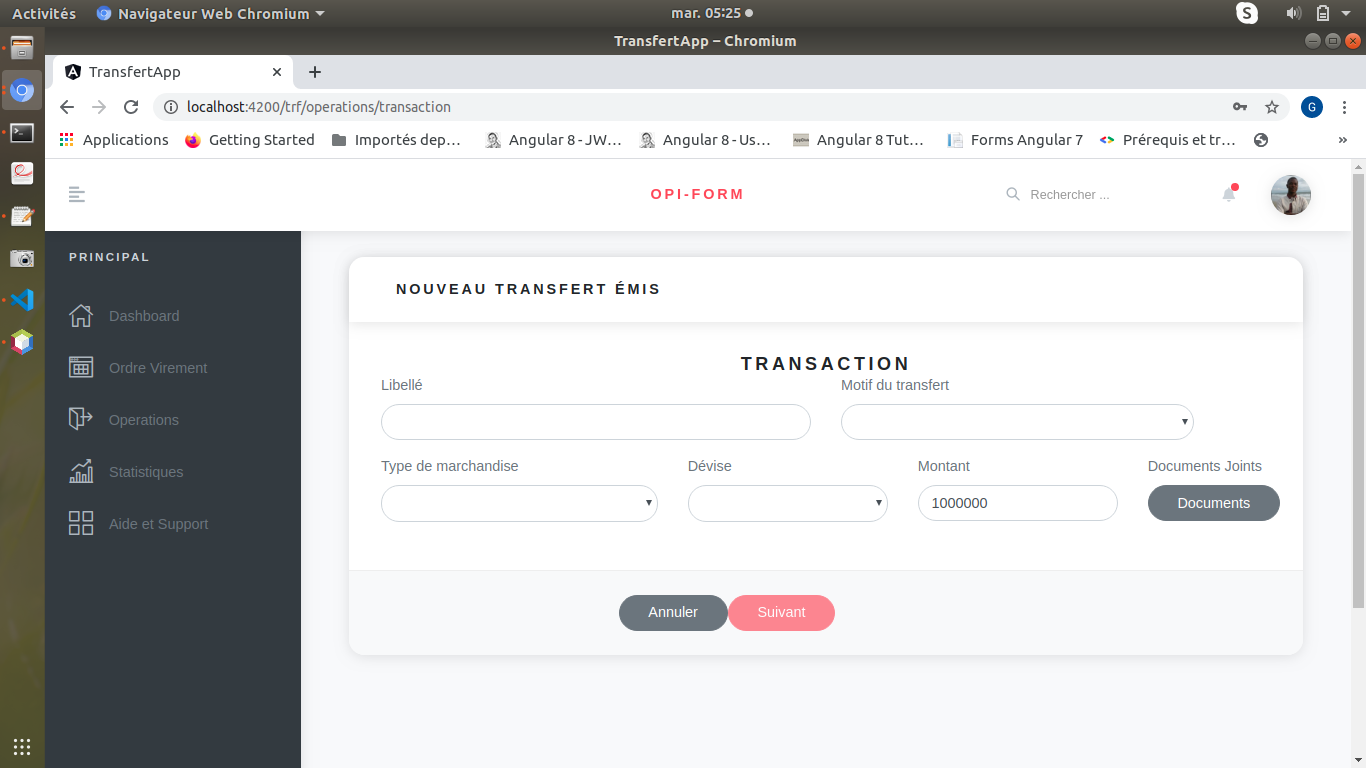
\includegraphics[width=14cm]{images/transaction.png}
    \caption{Ecran de renseignement des informations sur la transaction.\label{fig:transaction}}
  \end{center}
\end{figure}


\begin{figure}[h!]
  \begin{center}
    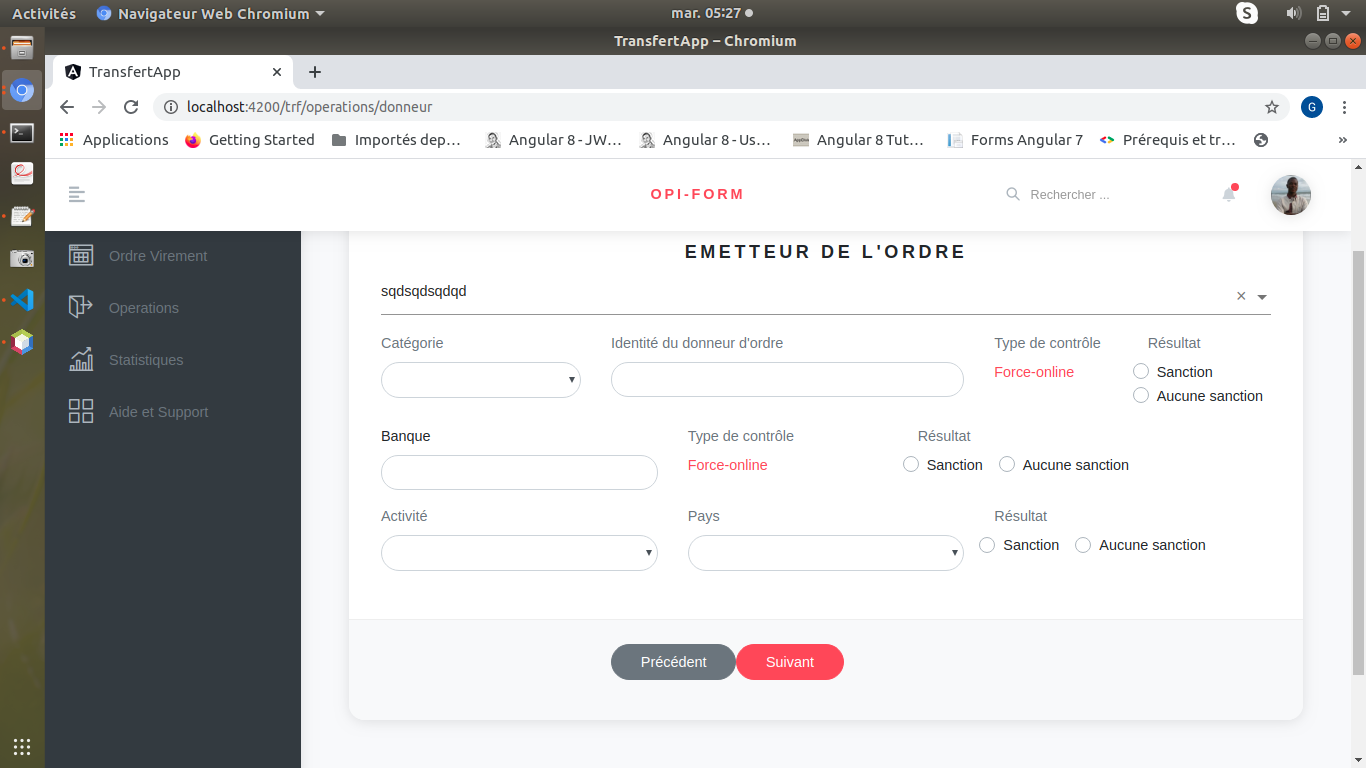
\includegraphics[width=14cm]{images/emetteur.png}
    \caption{Ecran de renseignement des informations sur l'émetteur de l'ordre.\label{fig:emetteur}}
  \end{center}
\end{figure}

\begin{figure}[h!]
  \begin{center}
    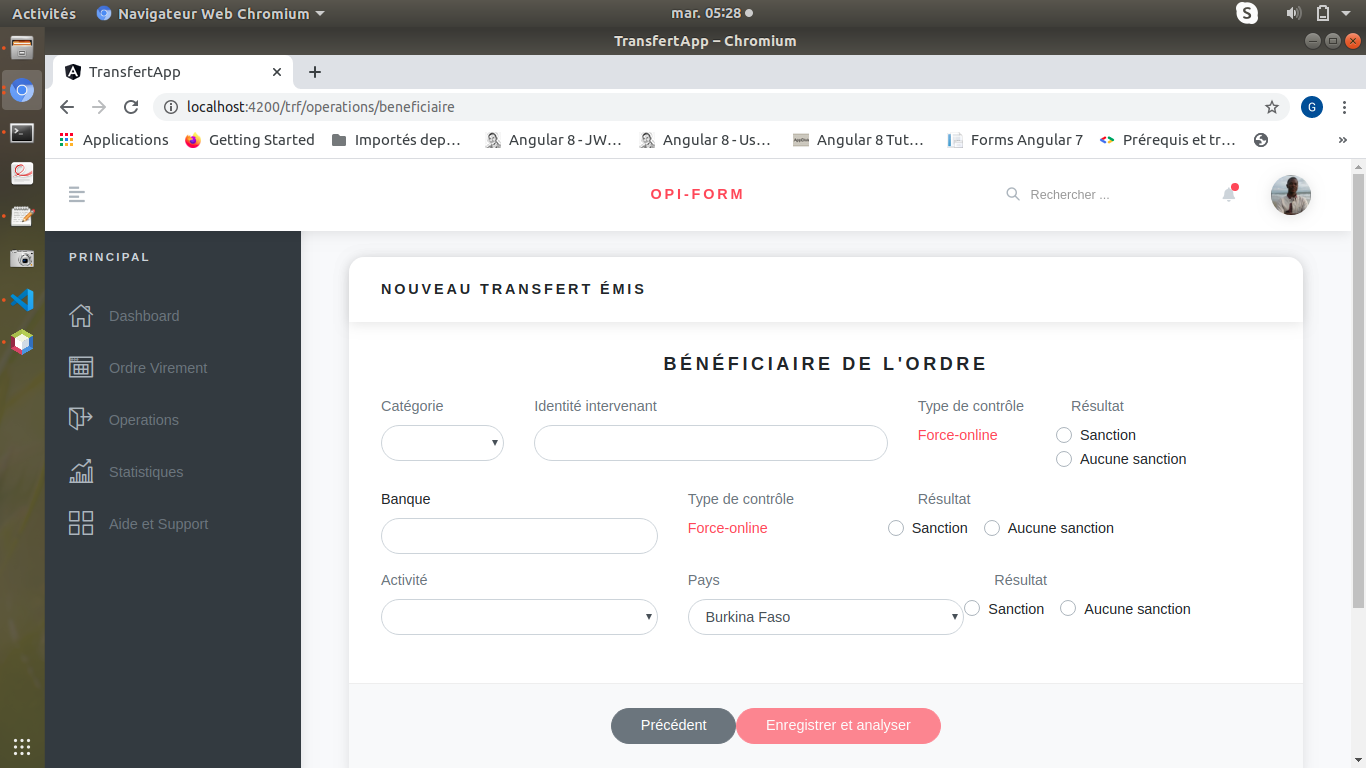
\includegraphics[width=14cm]{images/beneficiaire.png}
    \caption{Ecran de renseignement des informations sur le bénéficiaire de l'ordre.\label{fig:beneficiaire}}
  \end{center}
\end{figure}

\begin{figure}[h!]
  \begin{center}
    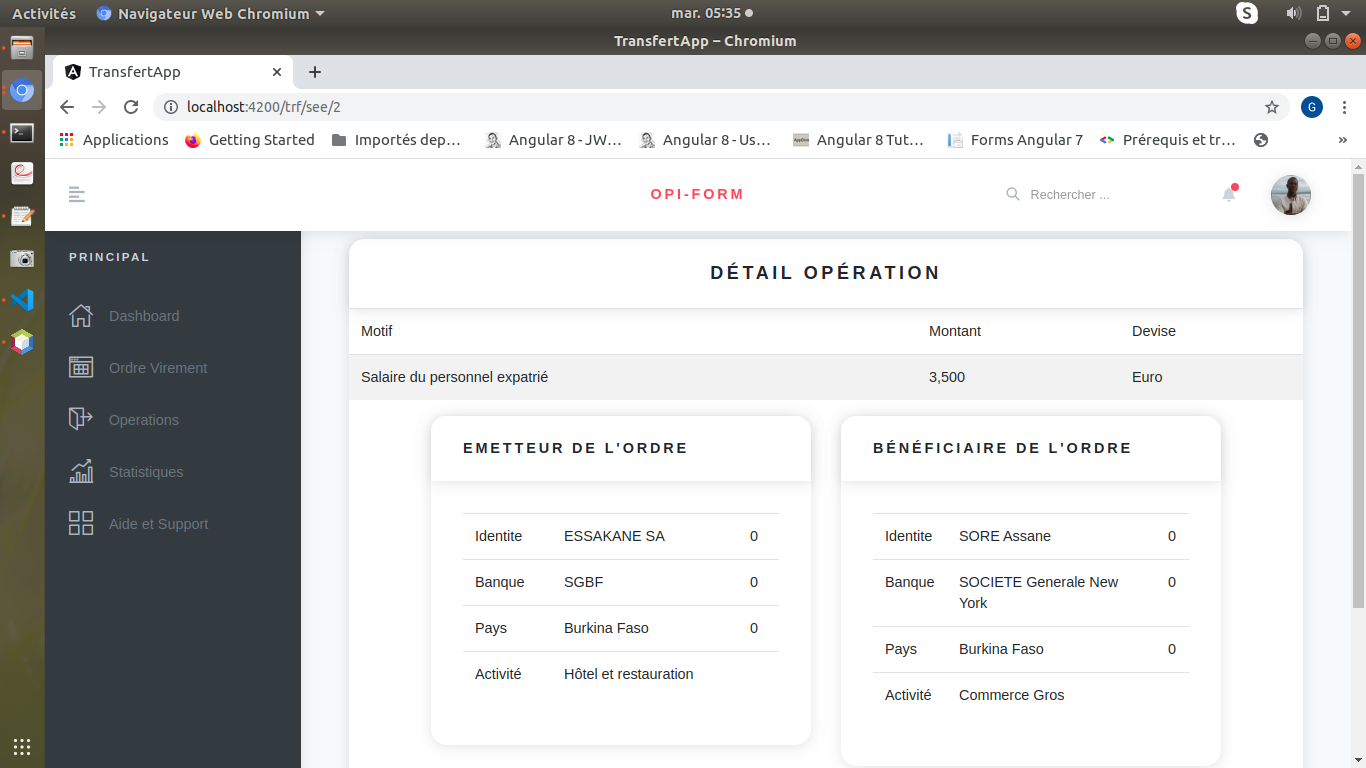
\includegraphics[width=13cm]{images/analyse.png}
    \caption{Ecran de présentation des détails et du résultat de l'analyse .\label{fig:analyse}}
  \end{center}
\end{figure}

   \section{Interprétation des résultats du modèle de machine learning}

  \subsection{Limites et difficultées}

  Sans passer par mille chemins, notre stage était miné de difficultés 
  d’ordre organisationnelles au sein de la banque et des difficultés 
  techniques rencontrées tous les jours.

  Les difficultés organisationnelles sont dues à l'acquisition et à la
  manipulation des données dont nous avions besoin pour l'implémentation de
  notre modèle. En IA, il est une barrière qui demeure impossible à franchir.
  \og Pas de datas, pas d'IA \fg. La principale difficulté a été l'obtention
  des données pour notre modèle. Les  modèles de machine learning se 
  construisent à partir d'exemples d'apprentissage basés sur l'expérience 
  passée. Disposer d'exemples est donc indispensable. Dans le même temps, ces
  exemples doivent être présents et suffisamment en grand nombre pour parvenir à
  une IA généralisable et applicable sur le terrain.

 Cette étape a été la plus difficile car elle a mis à contribution de nombreux 
 collaborateurs de plusieurs services différents(DCO, OPE). Cela nous a permis
 d'obtenir un jeu de données pour l'apprentissage.

  Les difficultés techniques sont liées au choix des différents outils
  d'implémentations du modèle, les pare-feux de la SGBF n'autorisant pas 
  l'installation de certaines applications sur les machines du réseau. Pour les
  outils dont l'installation était impossible, il fallait donc trouver d'autres
  permettant de faire la même tâche beaucoup plus difficilement.

    \subsection{Analyse des résultats}
 La matrice de confusion permet de résumer et visualiser les résultats d'un
 problème de classification. Des mesures permettent d'analyser la matrice de 
 confusion. Ce sont
 \begin{description}
   \item{La précision}: Elle permet de calculer le taux de classification juste.
     C'est la proportion des prédictions correctes parmi les points que l'on a
     prédit.
     $$
     Precision = \frac{VP}{VP + FN}
     $$
   \item{Le rappel ou sensibilité: } En anglais \textit{recall}, il donne la proportion des
     exemples bien étiquetés.
     $$
     Rappel = \frac{VP}{VP + FP}
     $$
   \item{L'exactitude: } En anglais \textit{accuracy}, il évalue le taux de
     bonnes réponses.
     $$
     Accuracy = \frac{VP + VN} {Vp + FP + VN + FN}
     $$
   \item{F1-score} Il s'agit de la moyenne harmonique de la précision et du
     recall. Il reflète les différents aspects du modèle.
     $$
     F1 = 2 * \frac{Precision * Rappel}{Precision + Rappel}
     $$
 \end{description}
   
 Les résultats obtenus après évaluation de notre modèle de classiication font
 ressortir quelques éléments.
 Globalement, la mesure du F1-score du modèle basé sur les arbres de décisions
 est d'environ 60\%. Les scores propres pour chacune de nos étiquettes montre
 une certaine différence. Le modèle prédit beaucoup plus facilement les dossiers
 non-conforme que les dossiers conformes. En effet le F1-score pour les dossiers
 non-conforme est approximativement de 93\% alors que celui des dossiers
 conformes est de moins de 86\%. cela pourrait être du fait que notre jeu de
 donnée contient plus de données d'opérations non conformes que d'opérations 
 conformes.
 
 Concernant l'exactitude de notre modèle,
 Peter Pan \cite{mediumPeter} obtenait un score 97\%  sur le dataset Iris.
 Le dataset iris est un jeu de données ouvert plusieurs fois cité dans la
 littérature. L'ensemble des données contient 3 classes de 50 instances 
 chacunes. Chaque classe se réfère à un type de classe iris.
 
 Jean philippe Vandamme et al. \cite{vandamme2006} ont mené une étude sur le taux d'échec en
 première année d'université. Ils ont essayé de prédire à partir de certains
 attributs qu'un étudiants puisse réussir son année(low-risk), réussir moyennant
 des actions menées par l'université(medium-risk) ou échouer(high-risk).
 Sur un ensemble de 533 étudiants questionnés sur un ensemble de 20 questions, ils ont obtenu un taux globale de
 bonne prédiction de 40,63\%. Ce taux est inférieur à celui que nous avons
 obtenu. 

 Ainsi, un volume plus important de données avec une répartition égale
pour chaque type de dossier permettrait d’atteindre des résultats plus beaucoup
plus satisfaisant. Néanmoins, les résultats obtenus sont prometteurs et nous 
permettent d'affirmer qu'il est possible d'utiliser du machine learning pour analyser
la conformité d'une opération à l'étranger.

\subsection{Perspectives}

L'analyse des dossiers d'opérations à l'étranger est une tâche fastidieuse. Le
modèle qui a été mis en oeuvre comporte de nombreuses imperfections.

\subsubsection{Concernant la diversité de nos données}

Pour notre modèle les données que nous avons utilisées relèvent de seulement vingt
cinq secteurs d'activités et 40 objets de transaction. Pour être efficace, le
modèle a besoin d'apprendre du plus grands nombres de secteurs d'activités et
également et de tous les objets de transaction de ces activités.


\subsubsection{Concernant le score de prédiction juste obtenu}

La conformité dans le domaine bancaire est très sensible. En effet, il s'agit
d'un domaine dans lequel l'erreur n'est pas autorisée. Une transaction
suspecte qui passe les mailles établies par la DCO entraine une cascade de sanction sur
l'institution financière en cause. Les structures bancaires ont donc besoin d'un
modèle qui puissent leur fournir un résultat très fiable. Ainsi notre score de
63\% de prédiction juste devrait être amélioré.

\section*{Conclusion}
Ce chapitre nous a permis de présenter l'implémentation du modèle
d'apprentissage automatique que nous proposons pour l'analyse des dossiers de
transferts. Les résultats que nous obtenons sont satisfaisants mais pourraient
être améliorés.


%------------------------------%
%------------------------------%
\chapter*{Conclusion Générale}
%------------------------------%
%------------------------------%
%\thispagestyle{plain}
\addcontentsline{toc}{chapter}{Conclusion générale}
\markboth{Conclusion}{Conclusion}

Le problème qui nous a été posé était l'application du machine learning dans 
l'analyse des opérations à l'étranger. De nombreuses opérations sont menées 
quotidiennement par la Société Générale Burkina Faso. Ces opérations sont 
délicates car engageant de nombreuses personnes: la personne qui émet 
l'opération, son correspondant bénéficiaire de l'opération, la banque émettrice
 et celle bénéficiaire et les nombreux intermédiaires.


L'expérience que nous avons mené durant nos 6 mois de stage à la Société Générale,
nous ont permis de comprendre le processus d'analyse et de mise en conformité 
d'une opération à l'étranger. Ce stage nous a également permis de détecter les
processus d'analyse qui peuvent être automatisés grâce à l'aprentissage 
automatique.


L'objectif de notre stage était de mettre en place une plateforme intelligente qui
permettrait d'analyser la conformité des dossiers de transferts déposés au guichet
de la société Générale Burkina Faso. La bonne réalisation de notre projet nous 
contraignait à une exploration dans l'univers des algorithmes de classification
afin de trouver celui qui répondait le mieux au spécification de notre 
problème. Notre choix s'est porté sur les arbres de décisions et c'est grâce à 
eux que nous avons réalisé notre projet.
Le jeu de donnée que nous avons utilisé pour entrainer notre modèle a été obtenu à
partir des dossiers physiques et grâce à la collaboration avec les membres  
des services impliqués dans le processus d'analyse du dossier d'une opération à
 l'étranger.


Le test d’évaluation de notre modèle a donné un score de 63\%. Les résultats obtenus
 mettent en évidence l’inégale répartition de nos données dans les différentes 
 classes. En effet, le modèle prédit mieux les opérations non conformes que 
 les dossiers conformes. Une seconde approche qui visera un approfondissement de
 notre modèle ne produira-t-elle pas de meilleurs résultats?



\appendix

\chapter{Annexe : Dossiers de transferts}

De nombreux documents entre en compte dans la constitution d'un dossier
d'opération à l'étranger. Dans cette annexe, nous présentons les principaux
motif d'opération à l'étranger et les documents composant le dossier. 

\section{Pour un règlement de facture d'achat}
Les documents constituant un dossiers pour une opération de règlement de facture
sont:
\begin{itemize}
  \item Un ordre de transfert précisant les coordonnées bancaires du
    bénéficiaire
  \item Une autorisation de change
  \item La facture réelle
  \item Une déclaration préalable d'importation(DPI)
  \item La facture proforma ayant servi à lever la DPI
  \item La facture définitive liée à la proforma ou à la DPI
  \item Une copie de l'attestation d'importation(AI SYLVIE) ou original si visée
    par la douane
  \item L'auorisation Spéciale 'Importation si produit spécifique
 \end{itemize}
\section{Pour le remboursement d'un emprunt}
Le remboursement d'un emprunt est une opération permettant de régler un prêt qui
avait été consenti auprès d'une banque ou d'un organisme. Les principaux
documents entrant dans cette opération sont:
\begin{itemize}
  \item Un ordre de transfert
  \item La convention de prêt
  \item Le tableau d'amortissement
  \item L'autorisation de change
  \item La preuve de rapatriement des dévises reçues
  \item La preuve d'encaissement des fonds au Burkina Faso
\end{itemize}

\section{Pour une prestation de service}
De nombreuses entreprises extérieures effectuent des assistances techniques au Burkina
Faso. Les documents permettant un transfert pour une prestation réalisée sont:
\begin{itemize}
  \item Un ordre de virement précisant les coordonnées bancaires du bénéficiaire
  \item La facture de prestation
  \item L'autorisation de change
  \item Le contrat de prestation de service
  \item La quittance de retenue à la source si la prestation est fournie ou
    utilisée au Burkina Faso
\end{itemize}


\section{Pour des frais de scolarité ou un soutien familial}
\begin{itemize}
  \item Un ordre de transfert précisan les coordonnées bancaires du bénéficiaire
  \item L'autorisation de change
  \item Un document attestant de l'inscription de l'étudiant pour
    l'année en cours ou de la présence du bénéficiaire à l'étranger.
\end{itemize}

\section{Pour le virement des salaires des personnes expatriés}
Les salaires des personnes de nationalité étrangères sont virés en dévises. Les
documents entrant en comptes dans une telle opération sont:
\begin{itemize}
  \item L'ordre de transfert précisant les coordonnées bancaires du bénéficiaire
  \item L'autorisation de change
  \item Le bulletin de salaire fait avec l'IUTS
  \item Le contrat de travail
  \item La copie du passeport
\end{itemize}






 
\chapter{Analyse et Conception de la plateforme Web}
 Nous présentons dans cette partie les phases d'analyse et de conception de
 l'application web. Il s'agira d'analyser le problème posé afin de concevoir une
 application répondant aux besoins qui ont été exprimés.

 \section{Analyse des besoins}

 Les besoins exprimés par la SGBF se résume en la mise en place d'un système
 permettant l'analyse vis à vis de la conformité d'un dossier de
 transfert déposé au guichet des opérations internationales. Partant de là, nous
 avons pu identifier les cas d'utilisations présentés dans le tableau
 \ref{tab:usecase}.

 Les principaux acteurs qui interagiront avec le système sont:
 \begin{description}
   \item[Le guichetier :] Il est chargé de la réception du dossier et de
     l'analyse de la cohérence et de la complétude du dossier. A la suite de
     cette analyse, il peut faire des observations sur le dossier.
   \item[L'administrateur :] Il a pour rôle la cration de nouveaux utilisateurs
     sur la plateforme. Il peut également consulter les statistiques.
 \end{description}
  \begin{table}
  \begin{center}
    \begin{scriptsize}
      \renewcommand{\arraystretch}{2}
      \begin{tabular}{|m{4cm}|m{10cm}|}
        \hline
        \rowcolor[gray]{.7}
        \bf \rule[-0.4cm]{0mm}{1cm} Cas d'utilisation &  \bf Description\\
        \hline
        Gérer un dossier & Enregistrer ou modifier un dossier. L'analyse
        conformité d'un dossier intervient juste après cette étape. \\ 
        \hline
        Faire des observations & Faire des observations sur la cohérence et la
        complétude du dossier \\
        \hline
        Gérer les accès au système & Création, modification et authentification
        des utilisateurs \\
        \hline
        Consulter des statistiques & Visualiser et exporter des données \\
        \hline
        Administrer le système & créer ou modifier les informations des
        utilisateurs. Attribuer des privilèges à un utilisateurs.\\
        \hline
      \end{tabular}
    \end{scriptsize}
    \caption{Les principaux cas d'utilisation du système \label{tab:usecase}}
  \end{center}
\end{table}

Le diagramme des cas d'utilisation résultant est le suivant. Il est présenté à
la figure \ref{fig:usecase}.

\begin{figure}[h!]
\begin{center}
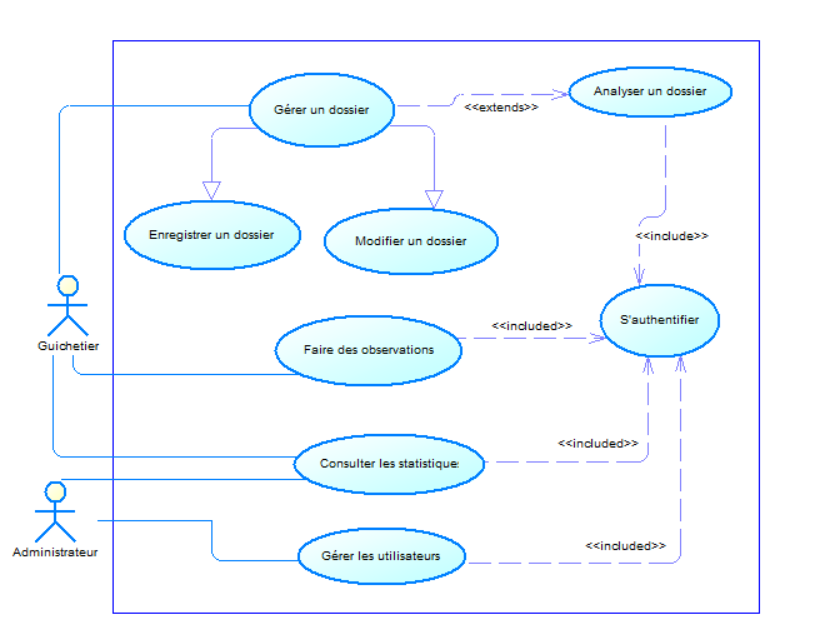
\includegraphics[width=14cm]
{images/usecase.PNG}
\caption{Diagramme des cas d'utilisation.\label{fig:usecase}}
\end{center}
\end{figure}
%


\begin{table}
  \begin{center}
    \begin{scriptsize}
      
      \begin{tabular}{|p{10cm}|}

        \hline
        Cas d'utilisation \og S'authentifier \fg\\
         \hline
         \uline{Titre: } S'authentifier \\
         \uline{Acteur Principal: } Guichetier \\
         \uline{Date de création :} 15/01/2020 \\
         \uline{Version: } 1.0 \\
         \uline{Auteur: } Ghislain Seghda\\
         \hline
         \textbf{Description des enchainements}\\
         \uline{Précondition}
         L'utlisateur dispose d'un ordinateur sur le réseau de la SGBF \\
         L'utilisateur dispose d'identifiant lui permettant d'accéder à la
         plateforme\\
         \hline
         \textbf{\uline{Scénario nominal}}\\
         \begin{enumerate}
           \item L'acteur se rend à l'adresse de l'application dans un
             navigateur depuis son ordinateur\\
           \item L'application se charge et présente la fenêtre
             d'authentification .\\
           \item L'acteur entre son nom d'utilisateur et son mot de passe puis
             valide ses entrées\[A1\], \[E1\]\\
           \item Le système vérifie l'authenticitédes informations et ouvre la
             page d'accueil.\\
         \end{enumerate}
         \textbf{\uline{Scénario alternatif}}\\
         \begin{enumerate}
           \item Le login et/ou le mot de passe sont incorrect pour la première
             ou la deuxième fois \\
           \item Le système informe l'acteur que les informations saisies sont
             incorrectes.\\
           \item Le scénario nominal reprend au point 1 \\
         \end{enumerate}
       \textbf{\uline{Scénario d'exception}}\\
       \begin{enumerate}
         \item L'acteur fourni pour la troisime fois des informations
           d'authentification erronées\\
         \item Le système bloque le compte de l'utilisateur\\
       \end{enumerate}
     \end{tabular}
   \end{scriptsize}
 \end{center}
\end{table}


\section{Conception}

Après l'identification des spécifications fonctionnelles du système, nous devons
procéder à sa conception. Pour y parvenir, nous avons suivi les étapes
suivantes:
\begin{itemize}
  \item Identification des entités ou concepts du domaine d'étude
  \item Identification et ajout des associations et des attributs
  \item Organisation et simplification du modèle en éliminant les classes
    redondantes
\end{itemize}
Le diagramme de classe obtenu est présenté à la figure \ref{fig:classe}.


\begin{figure}[h!]
\begin{center}
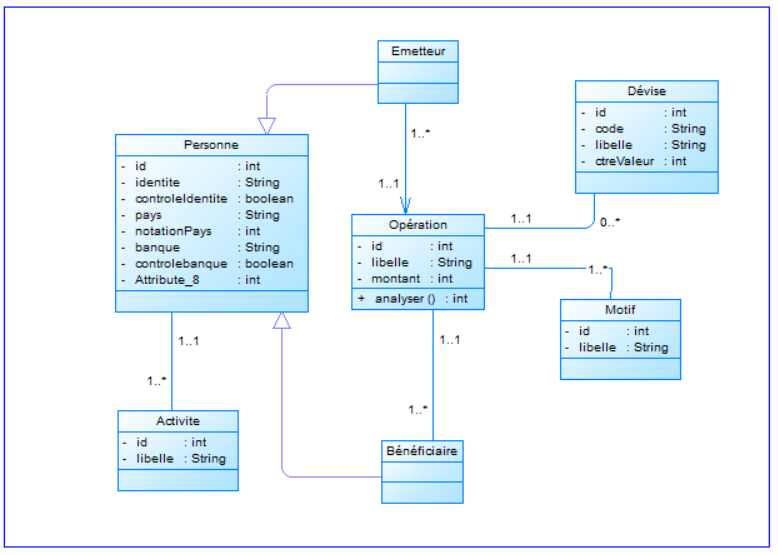
\includegraphics[width=14cm]
{images/classe.PNG}
\caption{Diagramme de classes.\label{fig:classe}}
\end{center}
\end{figure}



\printglossary

\bibliographystyle{plain}
%\nocite{*}
\bibliography{./biblio/all-refs}
\newpage
\end{document}
